%%%%%%%%%%%%%%%%%%%%%%%%%%%%%%%%%
% 6CCS3PRJ Final Year Individual Project Report
% luca-dorin.anton@kcl.ac.uk
%%%%%%%%%%%%%%%%%%%%%%%%%%%%%%%%%
\documentclass[11pt]{informatics-report}
\usepackage{color}
\usepackage[square,sort,comma,numbers]{natbib} %References
\usepackage{hyperref}
\usepackage{graphicx}
\usepackage{float}
\usepackage{pdfpages}
\graphicspath{ {./Images/} }

%%%%%%%%%%%%%%%%%%%%%%%%%%%%%%%%%
% Front Matter - project title, name, supervisor name and date
%%%%%%%%%%%%%%%%%%%%%%%%%%%%%%%%%
\title{6CCS3PRJ Background Specification Progress Report\\\vspace{0.2cm}Breadboard Computer Architecture}
\author{Luca-Dorin Anton}
\studentID{1710700}
\supervisor{Christian Urban}

\date{\today}

\abstractFile{FrontMatter/abstract.tex}
\ackFile{FrontMatter/acknowledgements.tex} %Remove line if you do not want acknowledgements

\begin{document}
\createFrontMatter
\onehalfspacing
\tableofcontents
\doublespacing

%%%%%%%%%%%%%%%%%%%%%%%%%%%%%%%%%
% Report Content
%%%%%%%%%%%%%%%%%%%%%%%%%%%%%%%%%
% You can write each chapter directly here or in a separate .tex file and use the include command.

\chapter{Introduction}
As the demand for high speed, low power, efficient and cheap computers rose over the past three decades,
manufacturers invested heavily into improving production processes, shrinking transistors, pipelining
instructions, creating new aggressive branch prediction models and implementing more and more functionality
into the hardware directly. Moore's prediction on the number of electronic components doubling on the
same surface area every two years held up well until recently when issues of quantum tunnelling started to
arise. This hasn't stopped the continuous enhancement of microprocessor and microsystems though. Now, instead
of making components smaller, manufacturers are installing more processing cores onto a single computing chip
package.
\begin{figure}[ht]
  \centering
  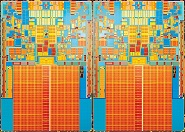
\includegraphics{45nm_quad_core_die}
  \caption{Intel quad-core 45nm CPU die}
  \label{intel_die}
\end{figure}
\linebreak
Another way of improving hardware is by implementing complex functionality, which would have been achieved traditionally through software, directly in hardware. An example of this is the implementation of the \emph{Advanced Encryption Standard} (AES) by \emph{Intel} directly in their lineup of CPUs through the \emph{AES-NI} instruction set extension \cite{aes2012ni}.
While the advantages for modern society of the continuous and accelerated development of hardware cannot be doubted,
there are also some worrying disadvantages. Such an advanced level of complexity in microprocessor design has been reached, that system and chip designers have started to increasingly rely on abstraction tools like \emph{ High-Level Synesthesis} to accommodate the advanced design requirements and meet user needs, as noted by Coussy in the \emph{User Needs} chapter \cite{coussy2008high}. On the one hand, this increasing complexity of hardware poses challenges for operating system and compiler developers, who need to constantly stay up to date with the newest improvements in the hardware space and integrate them into their products, to ensure user satisfaction and sustained quality over time. One the other hand, people, including developers, are presented with no need to understand the underlying machines with which they are interacting. To quote Bruce Scheiner, a famous cryptographer and computer scientist:
\begin{quotation}
People don't understand computers. Computers are magical boxes that do things. People believe what computers tell them. \cite{schneier2011secrets}
\end{quotation}
As a possible solution to this general human trend towards treating computers as ~~magical boxes'', this project proposes a simple and understandable \emph{practically implementable} machine architecture which has the same computational capabilities as a Turing machine. \linebreak
Some core features of the architecture are:
{\begin{itemize}
  \item 16-bit word length
  \item variable clock speed for live execution visualization
  \item single clock step function
  \item simplified input and output
  \item hardware addition and subtraction implementation
\end{itemize}}

The rest of the report will go through the steps involved in specifying, designing, building and testing the machine and the software to go along with it in great detail.
\pagebreak
\section{Inspiration and Motivation}
The main inspiration for this project is a YouTube series created by \emph{Ben Eater} titled \emph{~~Building an 8-bit breadboard computer!''} \cite{eater2019breadboard}. Eater's computer is itself a physical implementation of a theoretical
architecture called \emph{SAP-1}, which stands for \emph{Simple as Possible}. There are three variants of the SAP Architecture, SAP-1, SAP-2 and SAP-3, in inreasing order of complexity, all of which have been created by Malvino and Brown in their book \emph{Digital computer electronics} \cite{malvino1992digital}.
\begin{figure}[ht]
  \centering
  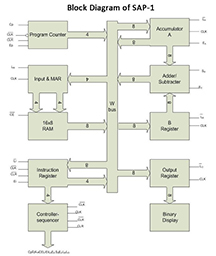
\includegraphics{sap1}
  \caption{Block Diagram of the SAP-1 architecture}
  \label{sap1}
\end{figure}
\linebreak
After going through the content, it became apparent that such a computer could serve as a great learning medium for developing a better understanding of computers, even more so with some hardware improvements and a sizable effort in writing some bespoke software for it. \emph{This project is largely based around Eater's design.} It serves not only as the motivational source for the project, but it also provides a solid foundation for which extension, enhancement and improvement can be within the scope of a final year project.

\section{Objectives}
The main goal of this project is the physical implementation of a 16-bit computer system modelled after an architecture designed around the ideas of \emph{explainability and ease of understanding} down to the transistor level. Breaking down this objective by specific hardware and software requirements, the following can be stated:
The main hardware  objectives are:
\begin{enumerate}
  \item 16 bit word length
  \item appropiatley sized memory space
  \item memory read/write capability
  \item capability to decode and execute instructions sequentially
  \item program counter alteration (jumps)
  \item I/O functionality
  \item hardware-implemented ability to perform basic arithmetical operations
  \item simple branching
  \item variable speed clock
  \item single step clock function
\end{enumerate}\pagebreak
The main software objectives are:
\begin{enumerate}
  \item adequate microcode for the control mechanisms
  \item assembly mnemonics
  \item assembler package to turn assembly files into binaries
  \item compiler for the WHILE-language to breadboard computer binaries
\end{enumerate}

\section{Project Structure}
The report begins with an in-depth circuit specification, design and analysis literature review. These core skills lay the theoretical foundation necessary for understanding the reasoning for choices when designing the hardware.
The next section is concerned with a detailed analysis of the computer built by Ben Eater \cite{eater2019breadboard}. Eater's computer serves as the template from which the design of the computer described in this report will originate. As such, it makes sense to analyse it carefully and classify its capabilities. \\
This will be followed by a specification of what the new computer should achieve in contrast to the capabilities of the existing computer. \\
The next chapter will cover the updated design of the computer. Important design decisions will be scrutinised and held against the main goals of the project. Both high-level, as well as in-depth design choices, will be taken into account. Main design challenges will be discussed and appropriate solutions presented. \\
After the design stage is complete, the following chapter will document the build phase. A detailed chronological breakdown of build progress will be presented. Testing will be executed in parallel with the building, so testing documentation will be found in this chapter as well. \\
With the build phase complete, the software development phase will follow. The design and implementation of the various software tools necessary for running the breadboard computer will be documented in this chapter.
With the software as well as the hardware ready, a rigorous testing phase will follow, coupled with an in-depth evaluation of the end product in comparison to the success criteria set at the start of the report. \\
Finally, the conclusion chapter summarises everything done so far and highlights the learning outcomes of the project and the possible continuation paths for future work. \\

\chapter{Background}
Since this project is largely focused around designing and building a new hardware architecture,
it is necessary to go through the existing material surrounding this topic. Hardware design can
be structured in many different ways. For the purposes of this report, a structuring based on increasing
abstraction levels will be used. Since the implementation objectives of the project aim to be educational in nature,
it is crucial to start off with as few assumptions about the existing systems as possible. As such, the following explanations assume zero previous knowledge. Besides this, the educational outcomes largely focus on developers and computer scientists, professionals who would benefit from a better understanding of the computer but who are not necessarily familiar with the field of logic design. As such, the definitions and explanations will be kept as brief as possible, to avoid possibly superfluous levels of detail.

\section{Computer Architecture}
Computer architecture refers to organization, functionality and implementation design details of a computer system. It can be generally split into two main categories: \emph{Instruction Set Architecture} and \emph{Microarchitecture}.

\subsection{Instruction Set Architecture (ISA)}
The \emph{Instruction Set} is the set of unique operations the computer is capable of performing. It is generally independent of the physical implementation of the system and it serves as an interface against which assembler, compiler and operating system designers and engineers can structure their products. ISA design will be a crucial part of this project. By building a hardware architecture from scratch, the opportunity for many different ISA design choices will present itself. Many of those choices will be presented, implemented and analysed in this report.

\subsection{Microarchitecture}
A computing system's microarchitecture refers to concrete and detailed implementation choices for the hardware which is to implement the Instruction Set defined through the ISA. For the purposes of this project, the microarchitecture design will come first, which will be done against a general set of requirements and then the ISA design will follow based on the hardware design choices made. The ISA design will serve as a stepping stone towards the software architecture stage of the project.

\subsection{General High-Level Architecture}
Generally speaking, all computers share some high-level design features:
\begin{itemize}
  \item \emph{A Processor,} or \emph{Arithmetic-Logic Unit (ALU),} which performs operations on some data
  \item \emph{A Memory} or \emph{Storage Unit,} which stores both data and instructions
  \item \emph{A Control Unit,} which decodes instructions and issues control signals
  \item \emph{Input/Output (I/O) devices,} to communicate with the outside world
  \item \emph{A Clock Pulse Generator,} which keeps all other modules running synchronously
  \item \emph{A Data Bus,} to facilitate the transfer of information between modules
\end{itemize}
Each individual component will be discussed in great detail in this report.

\begin{figure}[H]
  \centering
  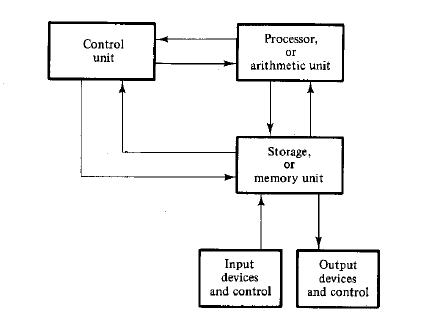
\includegraphics{comp_architecture}
  \caption{Block diagram of a digital computer, adapted from \emph{Digital Logic and Computer Design} by M. Morris Mano \cite{mano2017digital}}
  \label{comp_architecture}
\end{figure}

Figure \ref{comp_architecture} is a block diagram based on the previous listing of modules. The Data Bus is represented as the double-ended arrows connecting the different components together. The clock is omitted.

\subsection{The Processor}
The processor module is tasked with executing certain operations on data. Its mode of operation is only dependent on two inputs: the data to be operated on and the operation to be applied to that data. As such, the processor does not have to hold any kind of internal state; its output will always be the same for a certain input. This makes the processor a \emph{cobinatorial circuit}, meaning that it just implements some (albeit complex) logic function and does not have any internal state or memory.

\subsection{Memory}
Memory serves the purpose of storing data and instructions and returning the stored information when requested. By nature, it is a \emph{sequential} circuit, meaning that it has some internal state besides the logical function implementations used to communicate with the rest of the computer. Memory is organized in addresses, each address storing a word of information.

\subsection{The Control Unit}
The Control Unit oversees all other modules and ensures that everything is happening according to the present instruction. It also has the task of decoding the present instruction to correctly select the control signals which have to be issued next.
There are two main design choices to be made when constructing a Control Unit. One option is to \emph{hardwire} the logic. Whilst more efficient, this often proves to be tedious and very hard to alter. Another common and more accessible approach is the use of \emph{microcode.} Microcode control units use some sort of \emph{Read-Only Memory (ROM)} as a \emph{lookup table} to decide which control signals to switch on at a given time step of a given instruction. This lookup table is microcode. As it is implemented through a ROM, it can be easily reprogrammed or swapped out for a different ROM, making the maintenance of the Control Unit much more accessible.

\subsection{Input/Output Devices}
Input devices are used to inject instructions and data into the computer. Output devices communicate calculated results back to the user. I/O devices can take many forms and usually also require the computer to implement some sort of \emph{interrupt} system to notify the control logic that an external event is taking place. In the case of the computer built for this project, I/O devices will be abstracted as simple registers. The computer will read from and write to those registers.

\subsection{The Clock Pulse Generator}
Computers rely on a master clock to synchronise the activity of all other components. In modern microcomputers, this is usually accomplished through a \emph{crystal osscilator} which vibrates at a predetermined frequency. There are also other ways to achieve a steadily pulsating clock signal. In the case of the computer built in this report, a pair of voltage comparators will be used.

\subsection{The Data Bus}
Given a large number of modules present in a computer, it comes off as impractical to have each module communicate with each other module directly. In this situation, the data bus presents itself as an adequate solution. All modules connect both their input and their output terminals to the bus through some guard or buffer which allows them to disconnect from the bus as needed. Then, at any given clock pulse, only one device is allowed to connect and output to the bus, whilst any devices interested in receiving that information can connect and input from the bus. As long as only one device writes to the bus per clock cycle, the bus functions properly.

\subsection{Other Important Components}
Besides the main modules listed above, there are a few more components which are crucial to the optimal operation of a computer.

\subsubsection{Registers}
Registers are small memory units which can store only one word of memory. A computer system normally has a very limited amount of registers. In modern computers, registers have much shorter access times than memory. Besides storing data and programs, registers can have special functions, for example, input and output registers, registers tied to certain operations, flags registers and instruction registers.

\subsubsection{Power Supply}
Since the focus of this project is electrical computers, some sort of electrical power supply will be necessary. A simple solution for a power supply based on a mobile phone charger will be presented in a later section of the report.

\section{Implementing individual modules}
With the general architecture of a computer system in place, the next design step is to create and implement design for each individual module. This can be achieved by using circuit design theory and best practices.

\subsection{Types of electrical circuits}
Electrical circuits can be broadly classified into two main categories: \emph{combinatorial} and \emph{sequential} circuits. \emph{Combinatorial circuits} are circuits without any internal state (no memory) which implement a certain logic function. A logic function maps binary inputs to binary outputs. They are implemented as cascading layers of \emph{logic gates.} The main techniques which can be used to transform a logic function into a combinatorial circuit are standard form reductions, map creations and adequate use of don't care conditions (input/output conditions which are considered to be invalid/ will never happen). \emph{Sequential circuits} are composed of two parts:
\begin{enumerate}
  \item A memory structure usually built out of \emph{flip flops}
  \item One ore more combinatorial circuits, implementing some logical functions
\end{enumerate}

\subsection{Logic Gates}
Logic gates are electronic devices usually built out of transistors which perform certain logic functions.
A \emph{logic function} is a function which maps binary inputs to binary outputs.

\subsection{The Transistor}
A transistor is an electronic device which allows the control of the flow of one current source through a second, potentially smaller current source. This serves as the basic component for creating more advanced electronic components like logic gates.
\begin{figure}[h]
  \centering
  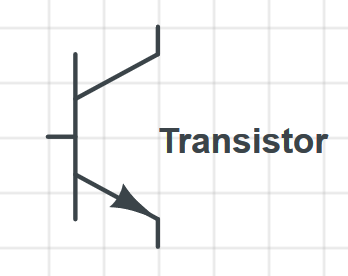
\includegraphics{trans}
  \caption{Transistor Symbol}
  \label{trans}
\end{figure}
Today, the most popular type of transistor and the most widley produced device in the world is the MOSFET \cite{chm2019mosfet}.


\subsection{Buffers}
Buffers are simple logic gates which just pass through the signal they receive.
\begin{table}[H]
\centering
\begin{tabular}{l|l}
\hline
\multicolumn{1}{|l|}{\textbf{A}} & \multicolumn{1}{l|}{\textbf{B}} \\ \hline
0                                & 0                               \\
1                                & 1
\end{tabular}
\caption{Truth table of a buffer}
\label{tab:buffer-table}
\end{table}
TO DO: ADD CIRCUIT DIAGRAM

\subsection{Inverters}
Inverters are similar in complexity to buffers. They invert the signal they receive.
\begin{table}[H]
\centering
\begin{tabular}{l|l}
\hline
\multicolumn{1}{|l|}{\textbf{A}} & \multicolumn{1}{l|}{\textbf{B}} \\ \hline
0                                & 1                               \\
1                                & 0
\end{tabular}
\caption{Truth table of an inverter}
\label{tab:inverter-table}
\end{table}
TO DO: ADD CIRCUIT DIAGRAM

\subsection{AND Gates}
And gates output a logic 1 only if all of their inputs are logic 1's.
\begin{table}[H]
\centering
\begin{tabular}{l|l|l}
\hline
\multicolumn{1}{|l|}{\textbf{A}} & \textbf{B} & \multicolumn{1}{l|}{\textbf{O}} \\ \hline
0                                & 0          & 0                               \\
1                                & 0          & 0                               \\
0                                & 1          & 0                               \\
1                                & 1          & 1
\end{tabular}
\caption{AND Gate Truth Table}
\label{tab:and-table}
\end{table}
TO DO: ADD CIRCUIT DIAGRAM

\subsection{OR Gates}
OR gates output a logic 1 if either of their inputs or both of them are logic 1's.
\begin{table}[H]
\centering
\begin{tabular}{l|l|l}
\hline
\multicolumn{1}{|l|}{\textbf{A}} & \textbf{B} & \multicolumn{1}{l|}{\textbf{O}} \\ \hline
0                                & 0          & 0                               \\
1                                & 0          & 1                               \\
0                                & 1          & 1                               \\
1                                & 1          & 1
\end{tabular}
\caption{OR Gate Truth Table}
\label{tab:or-table}
\end{table}
TO DO: ADD CIRCUIT DIAGRAM

\subsection{XOR Gates}
Exclusive OR, or XOR gates output a logic 1 only if either of their inputs is a 1, but not both.
\begin{table}[H]
\centering
\begin{tabular}{l|l|l}
\hline
\multicolumn{1}{|l|}{\textbf{A}} & \textbf{B} & \multicolumn{1}{l|}{\textbf{O}} \\ \hline
0                                & 0          & 0                               \\
1                                & 0          & 1                               \\
0                                & 1          & 1                               \\
1                                & 1          & 0
\end{tabular}
\caption{XOR Gate Truth Table}
\label{tab:xor-table}
\end{table}
TO DO: ADD CIRCUIT DIAGRAM

\subsection{NAND Gates}
A NAND gate is an inverted AND gate. This means it outputs a logic 1 in all situations except for when all of its inputs are logic 1's.
\begin{table}[H]
\centering
\begin{tabular}{l|l|l}
\hline
\multicolumn{1}{|l|}{\textbf{A}} & \textbf{B} & \multicolumn{1}{l|}{\textbf{O}} \\ \hline
0                                & 0          & 1                               \\
1                                & 0          & 1                               \\
0                                & 1          & 1                               \\
1                                & 1          & 0
\end{tabular}
\caption{NAND Gate Truth Table}
\label{tab:nand-table}
\end{table}
TO DO: ADD CIRCUIT DIAGRAM


\subsection{NOR Gates}
A NOR Gate is an inverted OR gate. This means it outputs a logic 1 only if all of its inputs are logic 0's.
NAND and NOR gates are considered \emph{universal gates}. This means that any logic circuit can be built exclusivley out of NAND or out of NOR gates.
\begin{table}[H]
\centering
\begin{tabular}{l|l|l}
\hline
\multicolumn{1}{|l|}{\textbf{A}} & \textbf{B} & \multicolumn{1}{l|}{\textbf{O}} \\ \hline
0                                & 0          & 1                               \\
1                                & 0          & 0                               \\
0                                & 1          & 0                               \\
1                                & 1          & 0
\end{tabular}
\caption{NOR Gate Truth Table}
\label{tab:nor-table}
\end{table}
TO DO: ADD CIRCUIT DIAGRAM

\subsection{Flip Flops}
Flip Flops are circuits usually built out of logic gates which can store one bit of information, i.e. they can be either on or off. There are many types of flip flops: RS-flip-flops (Reset-Set), D-flip-flops (Data), JK-flip flops (refined RS flip flops) and T flops (single input JK flip-flops). Each flip flop performs best in a certain scenario. Since they all implement de storage and retrieval of one bit of information, only the D-flip-flop (the most commonly used one) will be discussed. \\
TODO: ADD D FLIP FLOP DESC.


\section{8-Bit Computer Architecture Designed by Ben Eater \cite{eater2019breadboard}}
This section concerns itself with the detailed analysis of the 8-bit computer architecture designed by Ben Eater in his YouTube tutorial series \cite{eater2019breadboard}. This computer serves as the starting design for the computer discussed in this report in the later section, as such, it presents itself as a good topic for discussion.

\subsection{Main Features}
The main features of Bean Eater's 8-bit computer on a breadboard can be broken down as follows:
\begin{enumerate}
  \item 16 by 8 memory space (4-bit addresses, 8-bit words)
  \item adjustable and manually single-steppable clock
  \item two data registers: A and B
  \item ALU which implements addition, subtraction and simple branching based on zero and carry conditions
  \item Decimal output through three 7-segment displays
  \item Microcode-based control logic using \emph{EEPROMs} (electronically erasable and programmable read-only memory)
  \item Common 8-bit data and instruction bus
\end{enumerate}

\subsection{High-Level Overview}
\begin{figure}[ht]
  \centering
  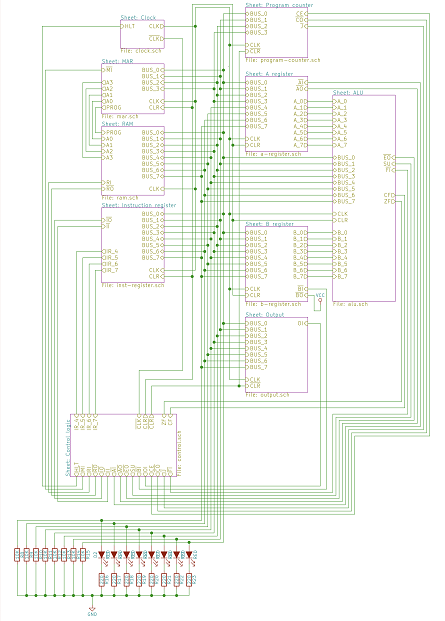
\includegraphics{8-bit-high-level}
  \caption{Block diagram of the 8-bit computer built by Ben Eater \cite{eater2019highlevel}}
  \label{8-bit-high-level}
\end{figure}



Figure \ref{8-bit-high-level} is a high-level block diagram displaying the inner workings of the 8-bit computer built by Ben Eater\cite{eater2019breadboard}. The following observations can be made when observing this diagram:
\begin{enumerate}
  \item Each module is connected directly to the common data bus. This means that every module can output information to the bus each clock cycle. After a judicious inspection of the microcode\cite{eater2019microcode} it is clear that no two modules output to the bus at the same time.
  \item The clock signal and the inverse clock signal are distributed throughout the computer to each module. Also, notice how there is a control signal for the clock as well. This \emph{HLT} (Halt) signal allows the computer to halt the clock, and implicitly halt the execution, for example after finishing a calculation, to allow it to be displayed.
  \item Besides the main connections through the bus, there are some additional \emph{special connections} between certain modules. For example, the \emph{A register} and the \emph{B register} have a direct connection to the \emph{ALU}, the \emph{MAR} (Memory address register) has a direct connection to the \emph{RAM} (Random Access Memory) and the \emph{IR} (Instruction Register) has a direct connection to the control logic.
  \item All control signals originate from the \emph{Control Logic} and spread out throughout the computer. Each module has at least one control signal
  \item This computer is severely limited in terms of memory. While 16 bytes can be sufficient for some demonstrational trivial programs (like Factorial or Fibonacci), it is insufficient for anything else.
  \item Another major limitation is the fact that it can only operate on signed integers. The architecture represents data in \emph{big endian, two's complement integer} format. No other data format or type is supported.
\end{enumerate}

\subsection{Module Design Conventions}
Ben Eater follows some essential design conventions when designing and building each of the modules for his computer.
The following subsections describe those conventions.

\subsubsection{Simplicity of understanding over cost and efficiency}

In many situations where a simpler solution from cost or efficiency makes itself notices, Eater often chooses to go for a more pragmatical approach which focuses on the simplicity of understanding. Since his computer mostly serves as an educational tool, it makes sense to pursue solutions which are easy to understand, over solutions which might be slightly cheaper or more efficient. A good example of this is in the design of the clock module \ref{eater2019clock}.

\begin{figure}[ht]
  \centering
  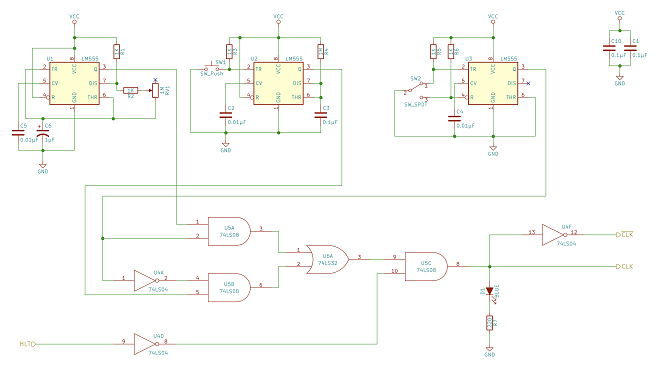
\includegraphics{8-bit-clock}
  \caption{Schematic of the clock module in Bean Eater's 8-bit computer \cite{eater2019highlevel}}
  \label{8-bit-clock}
\end{figure}

For the combinatorial circuit responsible for selecting a clock signal (either the automatic or the manual one) and also filtering out the clock when the \emph{HLT} (Halt) signal is active, Eater could have opted for a circuit built out of \emph{NAND} (Not And) gates instead of a circuit of AND, OR and inverter gates. This is because NAND gates are universal gates, which means that any combinatorial circuit can be built exclusively out of NAND gates. In this case, this would have had a net effect on cost, since the circuit could have been implemented with only two NAND ICs (integrated circuits), instead of three. The choice was made to use AND, OR and Inverter gates since the function of those gates is more intuitive and as such, the entire circuit is easier to understand.

\subsubsection{Connection to the Bus}

Eater's computer features an 8-bit common bus for both data and instructions. Most modules are tied to this bus directly. For the bus to function properly, only one device should be allowed to output to the bus at a time. Without some guards, connecting to the bus directly would mean that all modules would inadvertently drive the bus either high or low, depending on their output. The solution to this is the use of \emph{Tri-State buffer gates.} This gates can be set to be in three states, either on or off, depending on the signal passing through them, or in a \emph{high-impedance} state in which the two terminals of the buffer are essentially disconnected from each other. This is activated through a separate control signal. All modules which output to the bus do so through an IC (integrated circuit) containing such gates. An example of this can be seen on the A register \ref{8-bit-a-register}.

\begin{figure}[ht]
  \centering
  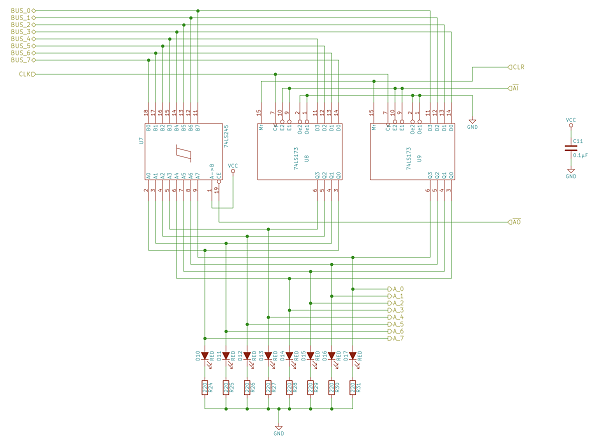
\includegraphics{8-bit-a-register}
  \caption{Schematic of the A register in Bean Eater's 8-bit computer \cite{eater2019highlevel}}
  \label{8-bit-a-register}
\end{figure}

% \chapter{Report Body}
The central part of the report usually consists of three or four chapters detailing the technical work undertaken during the project. {\bf{\textcolor{red}{The structure of these chapters is highly project dependent}}}. They can reflect the chronological development of the project, e.g. design, implementation, experimentation, optimisation, evaluation, etc (although this is not always the best approach). However you choose to structure this part of the report, you should make it clear how you arrived at your chosen approach in preference to other alternatives. In terms of the software that you produce, you should describe and justify the design of your programs at some high level, e.g. using OMT, Z, VDL, etc., and you should document any interesting problems with, or features of, your implementation. Integration and testing are also important to discuss in some cases. You may include fragments of your source code in the main body of the report to illustrate points; the full source code is included in an appendix to your written report.

\section{Section Heading}

\subsection{Subsection Heading}


A regular wall mountable phone charger usually provides around 1 Ampere of current at 5 Volts. A simple solution for a power supply is to take a phone charger with a detachable inexpensive \emph{USB micro-B} cable, remove the micro-B connector and solder breadboard pins onto the \emph{Gnd} (Ground) and \emph{Vcc} (+5V) pins. As such, an important consideration for hardware choice will be compatibility with a +5V power supply.

\chapter{Specification \& Design}
This chapter of the report focuses on creating a comprehensive set of specifications for the computer
to be built as a part of the project and then provides a detailed listing of the design choices made to satisfy
the specifications provided. Since the design will be based on Bean Eater's 8-bit breadboard computer \cite{eater2019breadboard}, but it will also include parts of SAP-2 and SAP-3 \cite{malvino1992digital}. Most specification criterions will be phrased as additions and enhancements to the existing designs.

\section{Specification Guidelines}
The specifications which are about to be presented serve the purpose of adding functionality to the 8-bit breadboard computer such
that its educational potential is harnessed more effectively, while at the same time avoiding over-complication and over-extensions
of scope. As such, it makes sense to list some of the features which will \emph{fall out of the scope} of this build for practical
and time considerations.
\begin{itemize}
  \item Interrupts and Interrupt handling
  \item Processes (The computer will only run one process, there will be no threading interface/ no operating system)
  \item Floating-Point operations
  \item Support for any kind of advanced in-hardware operations (for example encryption)
  \item Native support for signed integers over 16 bits
  \item Graphical User Interfaces (GUIs)
  \item Input through traditional peripheral (mouse and keyboard)
\end{itemize}

\section{Major Architecture Changes}
The computer should broadly follow the architecture o the 8-bit computer designed by Malvino and Brown \cite{malvino1992digital} and built by Bean Eater \cite{eater2019breadboard}. The major architectural difference should be \emph{the extension to 16-bit words}.
Since the word length of the computer should be 16 bits, its bus and most of its modules should be extended to accommodate this extra capacity.

\subsection{Operational Enhancments}
Besides Addition and Subtraction, the computer should also implement \emph{bit-shifting} (both left and righ). Bit-shifting is a crucial operation which is very often performed to increase the efficiency of certain operations (for example, multiplication and division by 2 can be expressed in binary as a left or a right shift of 1 bit)

\subsection{I/O Enhancements}
Currently, the only way to provide input to the 8-bit computer is by \emph{manually} programming each memory address through dip-switches. This is slow, clunky and prone to errors. There should exist a mechanism to quickly program the computer, for example through an external \emph{microcontroller} like an Arduino. Besides this, there should also exist a way for the computer to request input \emph{while executing} from an external device like a microcontroller.
Similarly, to provide persistence to the values from calculated by the computer, instead of being able to display only one value at a time, the computer should also have the ability to communicate with an existing external device like a separate microcontroller, providing it with the values it has calculated. In turn, the microcontroller a the be connected to a regular personal computer and then programmed to display those values to the screen. Besides this, the computer should have a display capable of displaying
more than 4 characters and more than just numbers.

\subsection{Stack Operations}
The addition of a stack pointer would make subroutines, calls to subroutines and callbacks significantly easier. An effective
stack pointer just has to have the option to increment and decrement, in contrast to a simple program counter which just increments.
With this functionality, return addresses can be pushed on and popped off of the memory stack whenever they are required.

\subsection{Expanded Random Access Memory}
Eater's implementation has a very limited address space (4 bit address, which equates to 16 addresses). While from a theoretical
point of view, this is as close to a Turing Machine as a supercomputer with terrabytes of RAM (an ideal Turing Machine should have infinite memory), a more reasonable amount of memory (in the kilobytes range) would allow for far greater flexibility in software
applications. For this computer, a 16K memory (\(2^10 * 16\), or 10 bit address space) should be sufficent.

\subsection{Memory Layout}
Due to the added features, the memory layout of the 16-bit breadboard computer needs to be re-worked. As such, the following
layout is proposed:
\begin{itemize}
  \item From 0x000 to 0x1FF: Program Text
  \item From 0x200 to 0x3EF: Variables and Data
  \item From 0x3F0 to 0x3FF: Stack
\end{itemize}

\section{16-bit Breadboard Computer Layout}
Based on the previous specification, the computer to be built in this report should contain the following modules and
have the following physical layout:

\begin{figure}[h]
  \centering
  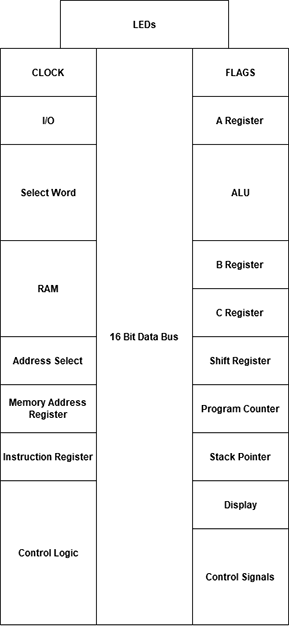
\includegraphics{16-bit-layout}
  \caption{High Level Module Overview and Layout of the 16-bit Breadboard Computer}
  \label{16-bit-layout}
\end{figure}
\clearpage

The updated computer specification contains the following modules, each of which will be followingly discussed in later sections:
\begin{enumerate}
  \item Common Data Bus \ref{common-data-bus}
  \item Data Bus LEDs \ref{data-bus-leds}
  \item Clock \ref{clock}
  \item A Register \ref{a-reg}
  \item B Register \ref{b-reg}
  \item Arithmetic-Logic Unit (ALU) \ref{alu}
  \item Flags Register \ref{flags}
  \item C Register \ref{c-reg}
  \item Shift Register \ref{shift-reg}
  \item Random Access Memory (RAM) \ref{ram}
  \item Program Counter \ref{pc}
  \item Stack Pointer \ref{stack-pointer}
  \item Display \ref{display}
  \item I/O \ref{io}
  \item Memory Address Register \ref{mar}
  \item Instruction Register \ref{ir}
  \item Word Selector \ref{word-select}
  \item Address Selector \ref{addr-select}
  \item Control Logic \ref{control-logic}
  \item Control Signals \ref{control-sigs}
  \label{module-list}
\end{enumerate}

\subsection{Common Data Bus} \label{common-data-bus}
The Common Data Bus acts as the communication medium of the computer. Drawing a parallel between \emph{computer design}
and \emph{human anatomy}, the data bus acts like the circulatory systems. It ensures all other components are connected
and can talk to each other. The Common Data Bus should be 16 bits wide, since the final system should have a word length of
16 bits. Since all other modules connect to the Data Bus, it makes sense to have it located centrally, between all other modules.
This way, no module has to have particularly long wires to interface with the Bus.

\subsection{Data Bus LEDs} \label{data-bus-leds}
This modules is as simple as it gets. It should be composed of just 16 LEDs, or Light Emitting Diodes, one on each Data Bus line,
so that whatever gets asserted at a certain point in time on the Bus can be visible. Besides this, it can also contain pull-down
resistors to ensure that, if no module asserts anything on the bus, it should default to low, or a logic 0.

\subsection{Clock} \label{clock}
The clock acts as the heart of the system. It provides a pulse under the form of a square wave, based on which all other components
do their job. The clock signal should be distributed to all other modules. Besides providing the square wave clock pulse an inverse,
or counter clock pulse should be available, as well as the ability to change the frequency and to completeley stop the square wave
and replace it with a manual button press for demonstrational and debugging purposes.
Finally, the clock should take in one signal as input, namely halt, or \emph{HLT},
which should completeley stop the clock regardless of operating mode. This will allow the computer to halt execution
if, for example, the program is finished. \\
\textbf{$Input Control Signals: HLT$} \\
\textbf{$Output Control Signals: CLK, \overline{CLK}$}

\subsection{A Register} \label{a-reg}
The A register is a 16-bit memory storage module. It should implement three functions. First, when its \emph{AI}
(A Register In) signal goes high, it should latch in the contents of the data bus on the rising edge of the next clock pulse.
The second function is to output its contents to the bus when its \emph{$\overline{AO}$} (A Register Out) signal goes low. Finally,
if the \emph{$\overline{RST}$} (Reset) signal goes low, it should clear out its contents and latch in a 0 on all bits. Additionally,
the A register should have a direct 16-bit connection to the \emph{Arithmetic Logic Unit}, or ALU \ref{alu}. \\
\textbf{$Input Control Signals: CLK, AI, \overline{AO}, \overline{RST}$}
\textbf{$Direct Connection to: ALU$}

\subsection{B Register} \label{b-reg}
Similarly to the A Register, the B Register should store 16 bits of data from the bus. It should have similar control signals,
\emph{BI, BO} and \emph{RST}, which perform equivalent functions. It should also have a direct 16-bit connection to the \emph{ALU}
\ref{alu}.
\textbf{$Input Control Signals: CLK, BI, \overline{BO}, \overline{RST}$}
\textbf{$Direct Connection to: ALU$}

\subsection{Arithmetic Logic Unit} \label{ALU}
The Arithemtic Logic Unit, or ALU, is the module responsible with data procesing. It takes the contents from\emph{both A and B
registers} \ref{a-reg} \ref{b-reg} directly and adds them up. Is the \emph{SU} (Subtract) signal is provided, the contents of the
B Register \ref{b-reg} will be subtracted from the contents of the A register. If the \emph{$\overline{\varepsilon O}$} (Sum Out)
is taken low, the contents of the  ALU will be asserted on the data bus. The ALU also has a direct connection to the Flags Register
\ref{flags}. Over this connection, the ALU should provide three flags:
\begin{itemize}
  \item Parity Flag: whether the \emph{Least Significant Bit} is 0 or 1
  \item Zero Flag: wheter the content of the ALU is 0
  \item Carry Flag: wheter the result of the operation of the ALU is cannot be expressed within 16 bits
\end{itemize}
\textbf{$Input Control Signals: \varepsilon O, SU$}
\textbf{$Direct Connection to: A Register, B register, Flags Register$}

\subsection{Flags Register} \label{flags}
The Flags Register is essential towards ensuring the Turing completeness of the computer being built. Based on the state of the
flags, the computer can make branch decisions, which reflect the fact that Turing machines can make selective decisions based
on the symbol it has just read.
Essentially, the flags register serves the purpose to latch in the three flags provided by the ALU \ref{alu}: the Parity Flag, the
Zero Flag and the Carry Flag. When the \emph{FI} (Flags In) signal is taken high, on the next clock pulse it should latch in the
contents of those flags. Besides this, the Flags Register should clear its contetns when the \emph{$\overline{RST}$} (Reset) signal
is taken low. There is a direct connection between the Flags Register and the Control Logic module, as the flags play a role in
deciding what to do next. \\
\textbf{$Input Control Signals: CLK, FI$}
\textbf{$Direct Connection to: ALU$}

\subsection{C Register} \label{c-reg}
The C Register serves as a general purpose 16-bit register. It has signals similar to the other two registers, A \ref{a-reg} and
B \ref{b-reg}. When \emph{CI} (C Register In) goes high, on the next clock pulse the register should latch in the data word
asserted on the bus in its storage. IF \emph{$\overline{CO}$} (C Register Out) goes low, the register should assert its contents
on the data bus. IF \emph{$\overline{RST}$} (Reset) goes low, it should clear its contents and latch in onyl zeroes. There should
be no direct connection between the C register and any other registers. \\
\textbf{$Input Control Signals: CLK, CI, \overline{CO}, \overline{RST}$}

\subsection{Shift Register} \label{shift-reg}
The Shift Register is the other module of the 16-bit breadboard computer capable of conducting data processing tasks. First and
foremost, it should act as a normal register, so it should latch in the bus contents on the next clock pulse if the \emph{SI}
(Shift Register In) signal goes high, asserts its contents to the bus if \emph{$\overline{SO}$} goes low, and clears it contents
if \emph{$\overline{RST}$} goes low. Besides this, if \emph{SFL} (Shift Left) goes high, on the next clock pulse it should shift its
contents to the left by one bit and insert a 0 at the least significant bit of the data word. Similarly, if \emph{SFR}
(Shift Right) goes high, on the next clock pulse it should shift its contents one bit to the right and insert a 0 at the most
significand bit of the data word. \\
\textbf{$Input Control Signals: CLK, SI, \overline{SO}, SFL, SFR, \overline{RST}$}

\subsection{Random Access Memory (RAM)} \label{ram}
Random Access Memory, or RAM, is the equivalent of the tape on a Turing machine. It can be read from and written to, and it should
be large enough to accommodate algorithms, data and variables; all at the same time. Memory is organised in addresses. Each address
should store one 16-bit word of memory. A 10-bit address is deemed to be sufficent, so the computer should have a
\(2^10*16 = 16K\) memory space. The RAM module should also have a direct connection to the \emph{Address Selector}
\ref{addr-select} and to the the \emph{Word Selector} \ref{word-select}. The Address Selector serves a 10-bit address to the
memory, while the word selector serves a 16-bit data word to the RAM. If the \emph{RI} (RAM In) signal goes high, on the next clock
pulse the RAM Module should latch in the data word served by the word selector at the address provided by the address
selector. If the \emph{RO} signal goes low, the RAM module should assert the data word stored at the address provided by the
address selector on the data bus. Additionally, based on two control signals originating from toggle switches, \emph{PROG} and
\emph{ARDUINO}, the signal which governs the RAM writes can be changed. If \emph{PROG} is low, that means the computer is in run
mode, and the \emph{RI} signal controls writes. If \emph{PROG} is high, then the computer is in programming mode, and the
write signal is chosen based on the \emph{ARDUINO} signal. If \emph{ARDUINO} is low, then the writes are manually controlled
using a simple push button. If it is high, then an external \emph{Arduino Mega} \cite{arduino2020mega} controls the writes to
memory using a signal called \emph{$ARDUINO_WRITE$}. \\
\textbf{$Input Control Signals: CLK, RI, RO, PROG, ARDUINO, ARDUINO_WRITE$} \\
\textbf{$Direct Connection to: Word Selector, Address Selector, Arduino Mega$}

\subsection{Program Counter} \label{pc}
The Program Counter serves the purpose of keeping track of the current address which should be executed. As such, it should
be a 10-bit register, to ensure coverage of the entire address space of the computer. If the \emph{CE} (Counter Enable) signal
goes high, on the next clock cycle the program counter should count up one in binary from the value it has currently latched
in its storage and then latch this new value in. If the \emph{$\overline{JMP}$} (Jump) signal goes low, on the next clock pulse the
program counter should latch in whatever value is asserted on the 10 loweest bits of the bus in its register. If
\emph{$\overline{CNT_O}$} (Counter Out) goes low, the value latched in the program counte should be asserted on the data bus.
If \emph{$\overline{RST}$} (Reset) goes low, the program counter should clear out its contents and latch in zeroes on all bits. \\
\textbf{$Input Control Signals: CLK, CE, \overline{JMP}, \overline{CNT_O}, \overline{RST}$}

\subsection{Stack Pointer} \label{stack-pointer}
Tha stack pointer should essentially be a register holding a 10-bit address, but accepting only a small subsection of the address
space (from 0x3F0 to 0x3F). This means that the stack should be 16 addresses tall. If the \emph{$\overline{ST_I}$} (Stack Increment)
signal goes low, on the next clock pulse, the stack pointer should increment by one. If \emph{$\overline{ST_D}$} (Stack Decrement)
goes low, the stack pointer should decrement by one on the next clock pulse.
On \emph{$\overline{ST_J}$} (Stack Jump) going low, on the next clock pulse the stack pointer should latch in the address asserted
on the bus in its register, assuming it is a valid stack address. If \emph{$\overline{ST_O}$} goes low, the stack pointer should
assert the address it has stored out on the bus. Finally, if \emph{$\overline{RST}$} (Reset) goes low, the stak pointer should reset
to zero. \\
\textbf{$Input Control Signals: CLK, \overline{ST_I}, \overline{ST_D}, \overline{ST_J}, \overline{ST_O}, \overline{RST}$}

\subsection{Display} \label{display}
The Display module is the main way through which the computer can interface with the user. It should have the ability to display
both alfanumeric characters and digits and it should feature at least 2 lines of 16 characters each. When the \emph{OUT} (Output)
signal goes high, the display should take a word of data from the bus and interpret it as the next character to be written to the
screen. \\
\textbf{$Input Control Signals: OUT$}

\subsection{I/O} \label{io}
Besides a display, the computer should also feature a bidirectional interface to another mirocontroller. In this case,
the interface should be to an \emph{Arduino Mega} \cite{arduino2020mega}. If the \emph{$\overline{E}$} (Enable) signal goes low,
based on the \emph{$R/\overline{W}$} (Read/Write) signal, the computer should interact with the Arduino. If the
\emph{$R/\overline{W}$} signal is high the computer should read a word of data from the arduino, so that word of data should be
asserted on the bus. If the \emph{$R/\overline{W}$} signal is low, the Arduino should read a word of data from the bus (and
consequently displayed to the user). \\
\textbf{$Input Control Signals: \overline{E}, R/\overline{W}$} \\
\textbf{$Direct Connection to: Arduino Mega$}

\subsection{Memory Address Register} \label{mar}
The memory address register, or MAR, is a 10 bit register. It connects directly to the address selector \ref{address-select} and
there is no other way to get the information latched into it. If the \emph{MI} signal goes high, on the next clock pulse the MAR
will latch into its storage the 10 least significant bits asserted on the bus. if \emph{$\overline{RST}$} goes low, the MAR will
clear its contents and write zeroas to all 10 bits. \\
\textbf{$Input Control Signals: CLK, MI, \overline{RST}$} \\
\textbf{$Direct Connection to: Address Selector$}


\subsection{Instruction Register} \label{ir}
The Instruction Register, or IR, is a 16-bit register which holds the next instruction to be processed. It is special in that
its most significant 6 bits have a different meaning. They represent the opcode for the current instruction and are directly
connected to the Control Logic module \ref{control-logic}. When the \emph{II} (Instruction Register In) signal goes high, on the
next clock pulse the instruction register should latch in the data word asserted on the bus in its storage. If the
\emph{$\overline{IO}$} (Instruction Register Out) signal goes low, the register should assert its least significand 10 bits to the
bus. If \emph{$\overline{RST}$} (Reset) goes low, the instruction register should reset and latch in zeroes on all 16 bits. \\
\textbf{$Input Control Signals: CLK, II, \overline{IO}$} \\
\textbf{$Direct Connection to: Control Logic$}


\subsection{Word Selector} \label{word-select}
The Word Selector is a special module, in that it serves the purpose of selecting between different sources of data and feeding
them into the RAM module \ref{ram}. There are three possible sources of data
\begin{enumerate}
  \item The Data Bus
  \item Dip Switches
  \item An Arduino Mega
\end{enumerate}
The Data Bus is the first and most straight forward data source. A 16-bit data word can be taken from the bus and then passed on
to memory. The second source are Dip Switches. Dip Switches are rows of small binary switches, which can be used to manually feed
binary data into a digital system. The last possible source of data is an arduino mega. The choice of data to be fed forward is
governed by two control signals, \emph{PROG} and \emph{ARDUINO}. If \emph{PROG} is low, data from the data bus will be selected,
regardless of the state of \emph{ARDUINO}. If \emph{PROG} is high, that means that the computer is in programming mode. In this
mode, the data source depends on the \emph{ARDUINO} control signal. If this signal is high, then data will be fed forward from
an external Arduino Mega \cite{arduino2020mega}. If it is low, then a series of 16 dip switches will be used to manually program
the computer.  \\
\textbf{$Input Control Signals: PROG, ARDUINO$} \\
\textbf{$Direct Connection to: RAM, Arduino Mega$}

\subsection{Address Selector} \label{address-select}
Similar to the Word Selector \ref{word-select}, the Address Selector selects between different address sources to provide a 10-bit
address to  the RAM module \ref{ram}. There are three possible data sources:
\begin{enumerate}
  \item The Memory Address Register \ref{mar}
  \item Dip Switches
  \item An Arduino Mega
\end{enumerate}
The choice of data source is defined by two control signals, \emph{PROG} and \emph{ARDUINO}. If \emph{PROG} is low, then the
computer is in run mode and the address latched in the \emph{MAR} \ref{mar} is fed forward to RAM. If it is high, then that means
the computer is in programming mode and the address choice is governed by the \emph{ARDUINO} control signal. If it is low, then
the memory address will be manually chosen using a series of 10 Dip Switches. If it is high, then an external
Arduino Mega \ref{arduino2020mega} will be the address source. \\
\textbf{$Input Control Signals: PROG, ARDUINO$}
\textbf{$Direct Connection to: RAM, Arduino Mega$}

\subsection{Control Logic} \label{control-logic}
To draw another parallel to human anatomy, the control logic module can be thought of as the ~~brain`` of the computer.
It takes in the 6-bit opcode from the Instruction Register \ref{ir}, the 3 flags from the Flags Register \ref{flags}, as well as
a 3 bit number representing the ~~step`` of the current instruction which is to be executed and decides based on these pieces
of information which control signals to keep active on the next clock cycle. It also maintains an internal 3 bit counter which
counts on the inverted clock or counter clock signal to provide the 3-bit step. \\
\textbf{$Input Control Signals: \overline{CLK}$}
\textbf{$Output Control Signals: HLT, \overline{RST}, AI, \overline{AO}, BI, \overline{BO}, \overline{\varepsilon O}, SU, FI, CI, \overline{CO}, SI, \overline{SO}, SFL, SFR, RI, RO, CE, \overline{JMP}, \overline{CNT_O}, \overline{ST_I}, \overline{ST_D}, \overline{ST_J}, \overline{ST_O}, OUT, \overline{E}, R/\overline{W}, MI, II, \overline{IO}$}
\textbf{$Direct connection to: Instruction Register, Flags Register$}


\subsection{Control Signals} \label{control-sigs}
The Control Signals Module is used to visualise which control signals are active at any given time. This module should
essentially consist of a labeled LED on each control signal.

\section{Specification Conclusion}
This concludes the specification phase of the project. The next step is to design each module to this specification.

\section{Design}
This section of the report focuses on the design process for the individual modules of the 16-bit breadboard computer.
The goal is to satisfy all specification criterions designated in the last section, while also adhering to the general goal
and philosophy of the project as close as project. First of all, the design process will be documented and analysed. After that,
the tools used to facilitate the design will be presented. Finally, each module design will be presented and scrutinized.

\subsection{How to design a 16-bit computer module}
In order to successfully come up with a design for a computer module while also meeting the specification outline and
keeping the schematics as simple as possible, a simple yet effective design process has been implemented. It consists
broadly of 4 distinct steps:
\begin{itemize}
  \item Chip Discovery
  \item Chip Analysis
  \item Chip Selection
  \item Schematic Creation
\end{itemize}

\subsection{Chip Discovery and Analysis}
The first step towards the design of a 16-bit computer module is the \emph{integrated circuit/IC/chip} discovery and analysis phase.

\paragraph{Why use Integrated Circuits/Chips?}
Since the general goal of the project is to produce a Turing complete computer which is as simple as possible to understand
and also relies as little as possible on any other form of abstraction, one might argue that using integrated circuits, or chips,
woud be against that goal. While this argument is theoretically correct, it doesn't take into account any practical considerations.
The lowest level of the technology stack from which one could go ahead and phisically construct a computer would probably be
the transistor. That being said, trying to implement any computer, let alone a 16-bit computer with many different modules, would
be next to impossible to successfully do within the time frame of this project and also without a team of people. The physical
scale would be many, many times what the scale of the computer built in this project is and the amount of errors which would arise
from connecting individual transistors together by hand would probably be so large, that one would quickly lose interest in
finishing the build. As such, simple integrated circuits pose themselves as a great compromise. These circuits, which usually
implement simple logic functions, like \emph{AND, OR, Inverter, etc.}, or even a little bit more complex functions,
like \emph{registers or binary adders}, can each contain tens to hundreds of individual transistors. That being said, they should
all be simple enough so thatthe functionality provided by each chip should be \emph{understandable down to the transistor level}.

\paragraph{Understanding Integrated Circuits}
While this may sound daunting at first, it can actually be relatively straight forward. Individual logic gates are each made up of
a few transistors. For example, Ben Eater has created an excellent YouTube tutorial on how to create logic gates out of transistors
\cite{eater2015logicgates}. Armed with this knowledge, we can now approach the datasheet of a particular circuit we intend to use.
For example, on page 2 of the datasheet of the \emph{74LS157} \cite{74ls157} multiplexer chip, we can find the logic diagram.
By analysing the logic diagram and calculating boolean outputs based on arbitrary inputs and then comparing the results
to the truth table of the chip provided on the first page of the datasheet, one can verify that the chip actually implements its
specified interface in a logical manner. This can be applied to all chips which are considered to be potential building blocks
for a module, as long as the individual chip complexity is relatively limited.

\subsection{Where to look for Integrated Circuits}
There are three main sources of chips which where consulted when conducting chip discovery. The first one was the Wikipedia list
of chips from \emph{7400} family \cite{wikipedia74lslist}. This particualr logic family was chosen because it is the most popular
and widley spread and adopted logic family in the world \cite{wikipedia74ls}. The second souce of chips, which served as a quick
reference, was Eater's part listing for his 8-bit breadboard computer build \cite{eater2020parts}. Since the 16-bit computer which
is to be built is largley based around the 8-bit computer built be Eater, many of the chips used in the 8-bit version will also
work in modules of the 16-bit version. Finally, for the few chips which were needed but weren't part of the 7400 family,
the websites of the retailers from which the chips were to be bought were searched. Two retailers were used, \emph{Mouser UK}
\cite{mouser} and \emph{Farnell UK} \cite{farnell}.

\subsection{Chip Selection}
Usually, the particular functionality of the module which is to be designed drastically boils down the list of potential chips.
For example, when designing a simple 16-bit register, like the \emph{A register} \ref{a-reg}, the \emph{74LS273} 8-bit flip-flop
\cite{74ls273} poses a great option. By just putting two \emph{74ls273} chips next to each other, most of the functionality of the
register has been designed. Whenever there is a need for extra functionality, for example in the case of the \emph{74ls273}
where there is no enable line, additional logic can be implemented using chips containing simple logic gates, like \emph{AND, OR,
NOT}. In this case, the clock signal can be AND'ed together with the \emph{AI} line to ensure that the register only reads from the
data bus when the control signal is set high.

\subsection{Schematic Creation}
With the right chips chosen for a module, the next step is to create a module schematic, which serves as a blueprint or design
document. The open-source computer-aided design software chosen to facilitate the creation of module schematics is \emph{KiCad}
\cite{kicad}. An overview of the application, as well as of the process of designing 16-bit computer modules with it will be
presented in detail in the next section.

\subsection{Electornic Design Tools with KiCad/Eeschema}
The main tool used to to design schematics for the 16-bit breadboard computer is \emph{KiCad} \cite{kicad}. KiCad is a broad and
mature electronics design software widley used in industry. It contains many tools which together from a tightly integrated
toolchain for designing complex electronics from the concept phase all the way to the printed circuit board. Since the goal of the
project is to build a computer on breadboards by hand and not create printed circuit boards, only the first step of the KiCad
pipeline has been used, namley \emph{Eeschema} \cite{eeschema}.

\paragraph{Eeschema}
\emph{Eeschema} is a electronic schematic computer design software. It is fully featured, easily accessible and has a relatively
shallow learning curve. By using \emph{Eeschema,} the entire module design process has been streamlined significantly.

\begin{figure}[h]
  \centering
  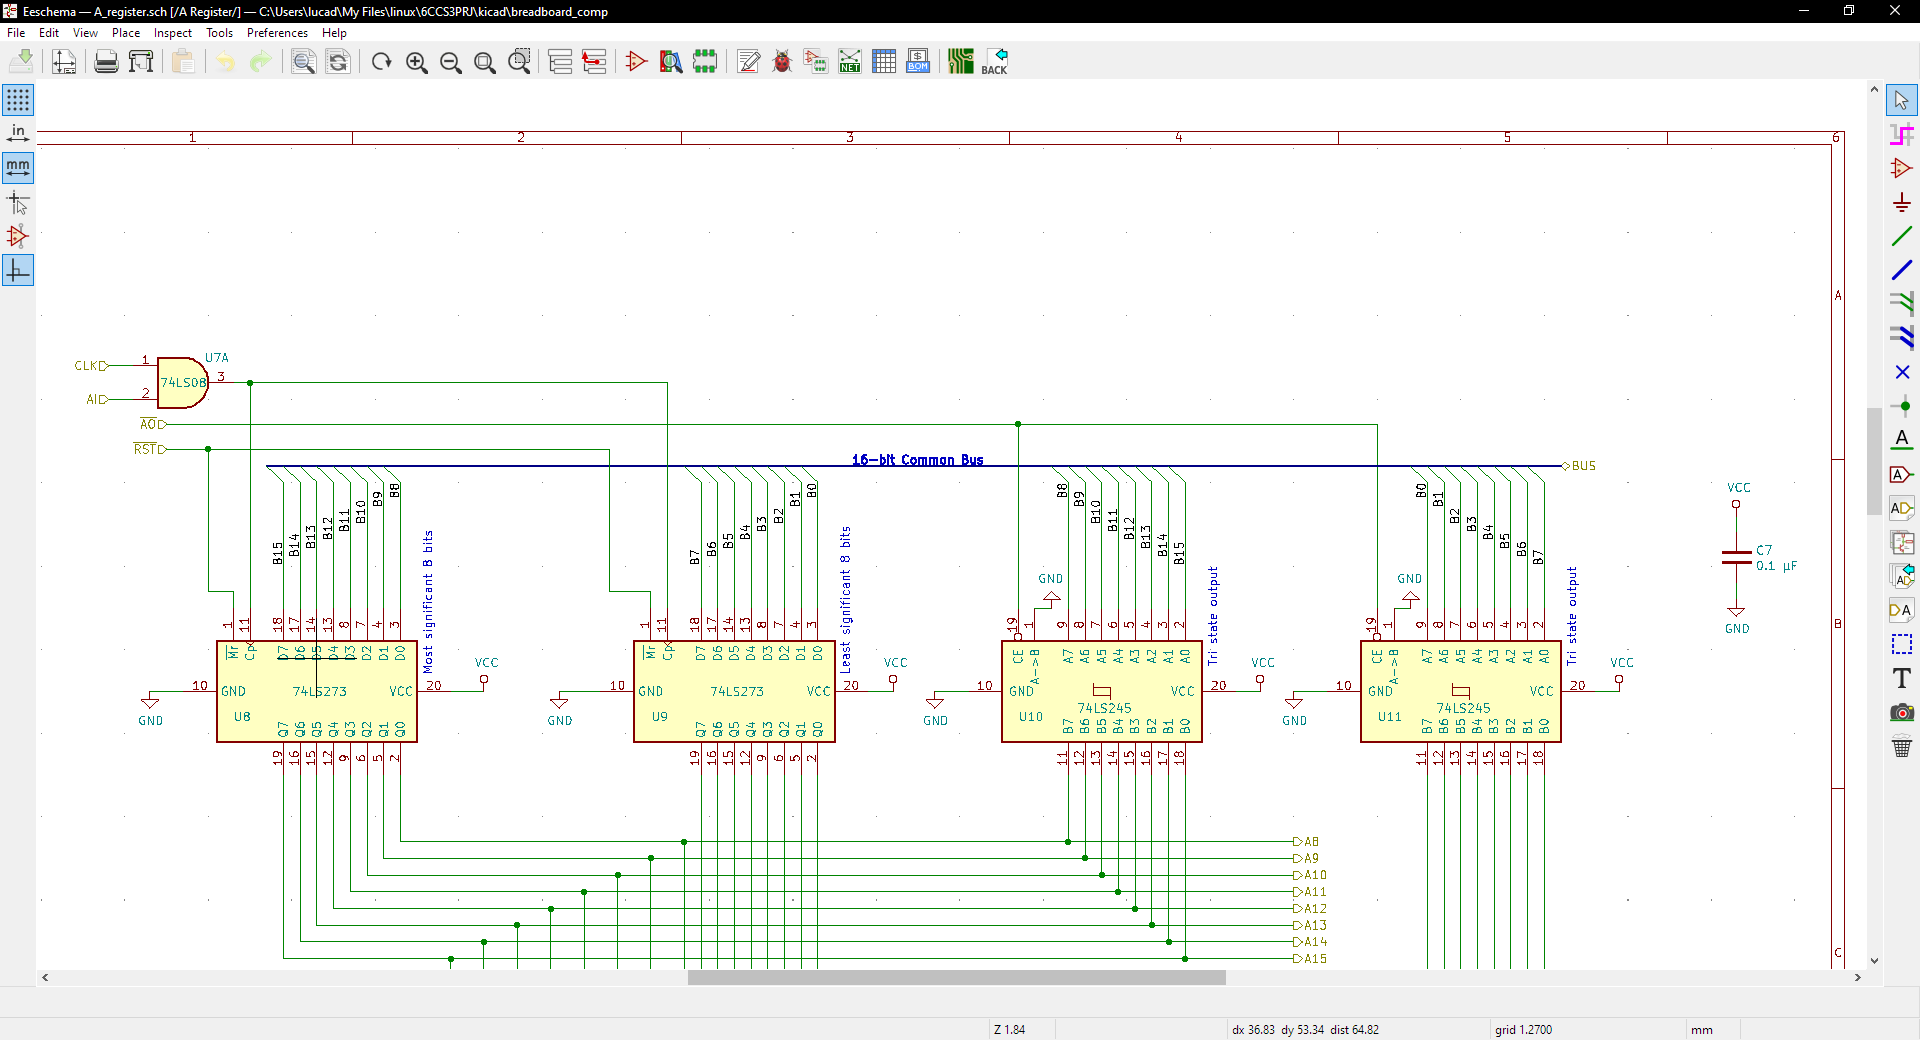
\includegraphics{eeschema}
  \caption{Eeschema Schematic Design software - part of the KiCad suite}
  \label{eeschema-interface}
\end{figure}
\clearpage

In the following paragraphs the most important features of Eeschema will be presented.

\paragraph{Intuitive Interface}
The graphical user interface provided by Eeschema is similar to many other widley used photo or video editing software packages.
As such, navigation is easy and intuitive. All tools and commands can be accessed both by pointer and keyboard, so one can become
proficient in whatever interface method is preferred. Drag and drop functionality allows the user to easily reposition misplaced
or misalligned circuits and components.

\paragraph{Hierarchical Sheets}
Hierarchical sheets is an Eeschema feature which allows one to embed entire schematics inside other schematics and seamlessly
transition between child and parent schematics. This is a great way to organise the modular design of the 16-bit breadboard
computer. Besides this, Eeschema offers the option to import input and output pins from the child schematic into the parent,
so that they can be connected to the wider circuit. This makes designing a high-level overview diagram significantly easier.

\paragraph{Bus connections}
Wiring up 16 separate wires which are connected to most modules as both input and output can be extremley tedious. Fortunatley,
\emph{Eeschema} offers the option to ~~bundle up'' mutliple wires as a single Bus and then have connections going in and out
of that single wire. Besides this, \emph{Eeschema} can resolve which pins are connected to which over the bus by use of labels
on the inputs and outputs \ref{ee-bus}.

\begin{figure}[h]
  \centering
  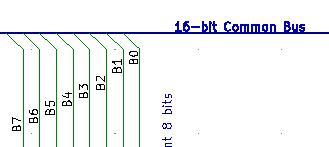
\includegraphics{ee-bus}
  \caption{Labeled Bus Connections in Eeschema}
  \label{ee-bus}
\end{figure}

\paragraph{Integrated Circuit Database}
\emph{Eeschema} ships with a pre-loaded database of commonly used chips and circuits, called the \emph{Symbol Library}.
This makes rapid schematic prototyping possible by just looking up potential circuits for the module and then dragging and dropping
them into the worksheet and then seeing if the connections would match up.

\begin{figure}[h]
  \centering
  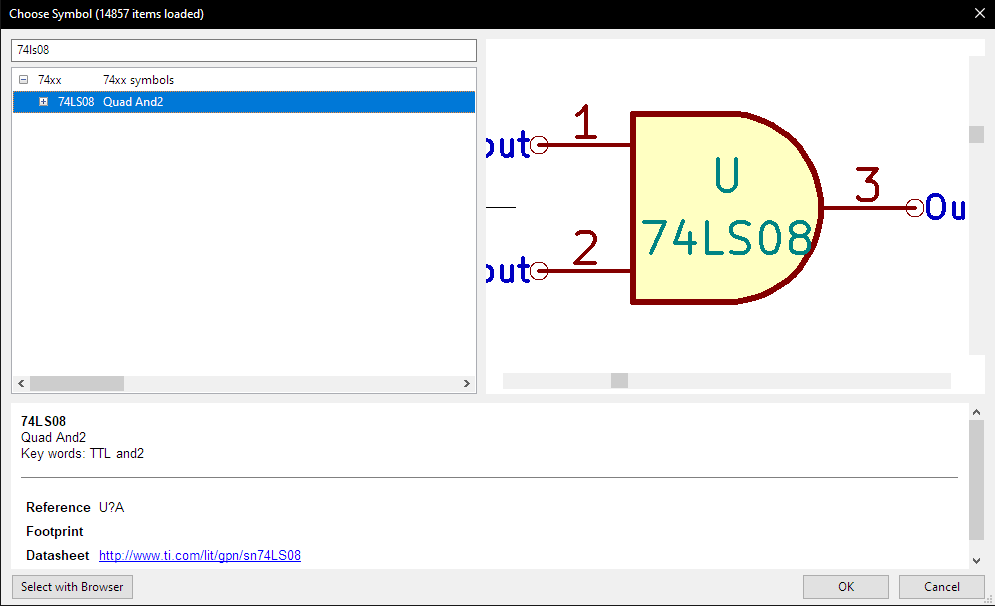
\includegraphics{ee-circuit-db}
  \caption{Component Database in Eeschema}
  \label{ee-circuit-db}
\end{figure}

\paragraph{Sympbol Editor}
In the rare case where the \emph{Symbol Library} didn't contain a circuit needed for a module, \emph{Eeschema} provides
a simple circuit symbol editor. This ensures that the final schematics produced were accurate and reliable, regardless of wherer
the chip symbols were origianlly available in \emph{Eeschema} or not.

\begin{figure}[h]
  \centering
  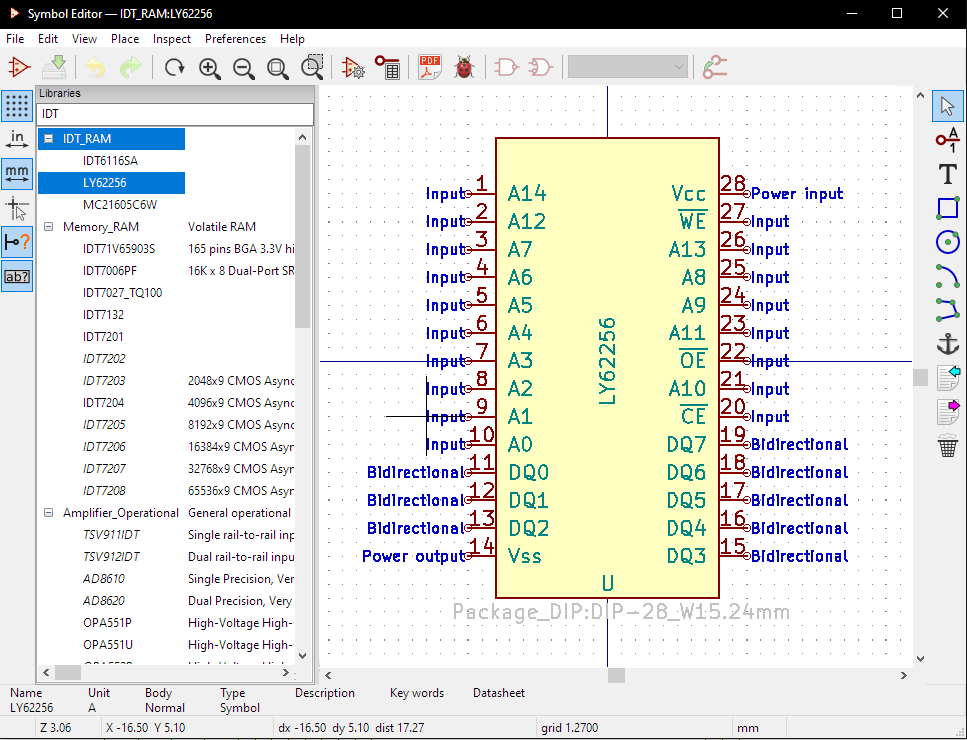
\includegraphics{ee-editor}
  \caption{Symbol editor in Eeschema}
  \label{ee-editor}
\end{figure}

\paragraph{Electrical Rules Check}
Besides providing an easy to use interface for designing accurate schematics, \emph{Eeschema} also offers active help in the
design process. By using the electrical rules checker, \emph{Eeschema} can check all connections against a user-defined set of
rules and report errors. This can be used to detect potetential human errors or even chip incompatibilities and resolve them
early on.

\begin{figure}[h]
  \centering
  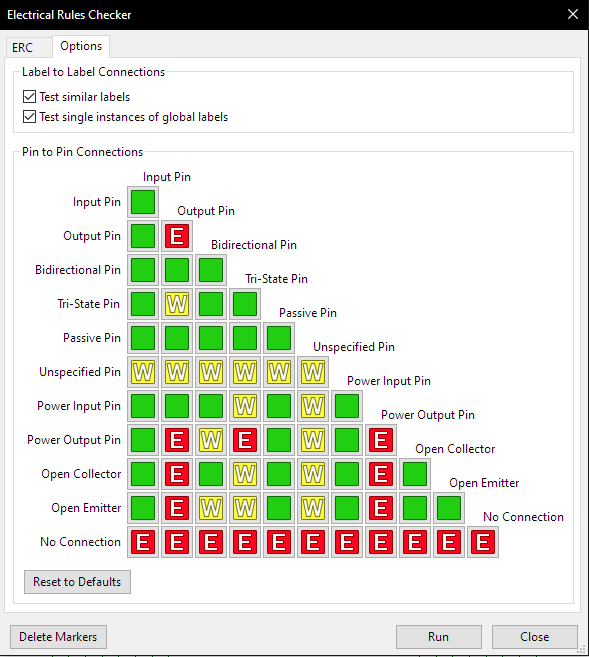
\includegraphics{ee-rules}
  \caption{The Eeschema Electrical Rules Checker}
  \label{ee-rules}
\end{figure}

\paragraph{Automatic Annotation}
When designing electrical circuits, it is common to use many identical or similar circuits next to one another. As such,
when actually building the circuit, one can be confused about which chip correlates to which symbol in the schematics.
To solve this, \emph{Eeschema} assignes a unique identifier, or annotation, to each symbol. This annotation process can be
done automatically.

\paragraph{Bill of Materials}
\emph{Eeschema} can also generate a bill of materials, or \emph{BOM}, based on all the symbols present in the schematic and
hierarchical schemaitcs. The BOM is essential towards ensuring that all needed components are purchased.

\begin{figure}[h]
  \centering
  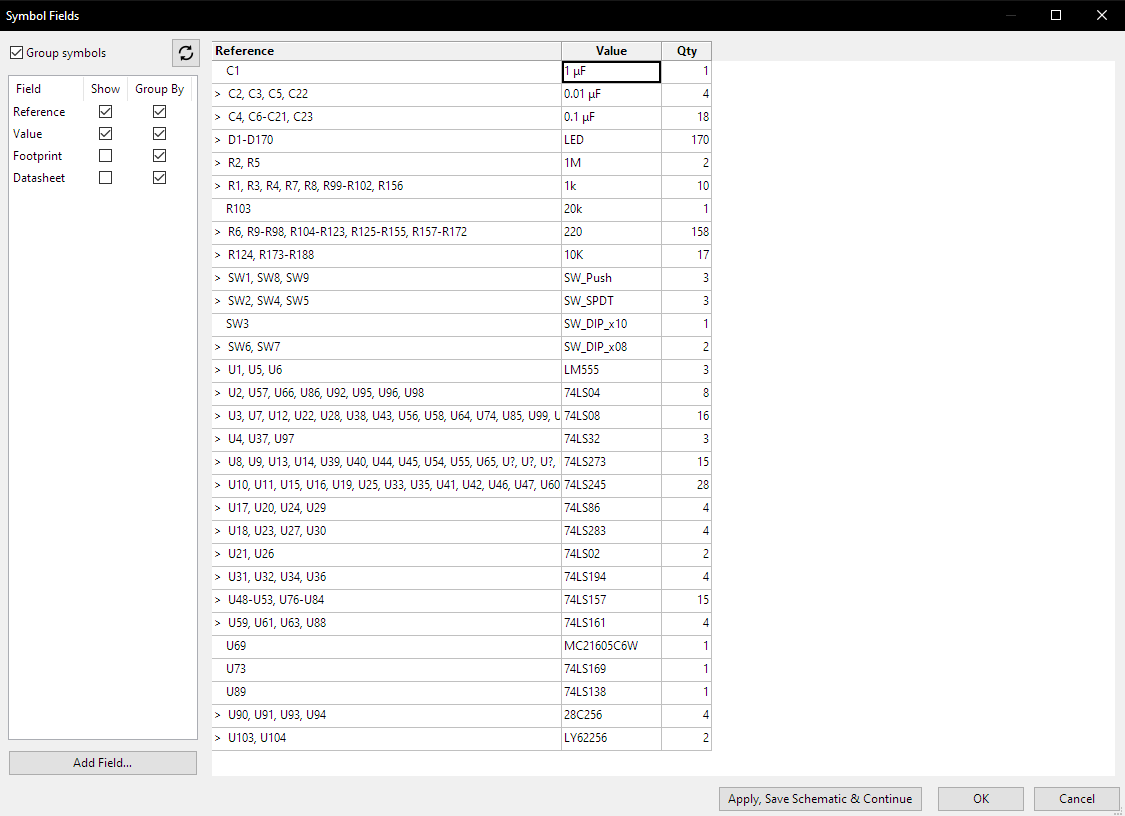
\includegraphics{ee-bom}
  \caption{Simple Bill of Materials generated by Eeschema}
  \label{ee-bom}
\end{figure}

\paragraph{PDF export}
Finally, Eeschema has been outfitted with an ~~Export to PDF'' option. This makes printing and compiling of the
schematics into other documents, like this report, significantly easier.

\subsection{Eeschema Design Process}
The following design process has been followed when creating schematics for a module as a part of the 16-bit breadboard
computer:
\begin{enumerate}
  \item Make an adequate chip selection
  \item Create a new hierarchial sheet and enter it
  \item Use the Symbol Editor to create chip symbols (in case the chips don't exist in the Symbol Library)
  \item Place all needed chips in the schematic
  \item Place all external control and I/O pins
  \item Connect all the pins apropiateley
  \item Leave the hierarchical sheet and import all I/O and control pins
  \item Run the automated annotation tool
  \item Run the electrical rules checker
  \item Correct any errors
\end{enumerate}

\subsection{Finalised 16-bit breadboard computer design and schematics}
The tools and processes discussed in the previous sections where extensivley used to produce the final schematics
for the 16-bit breadboard computer, which were used as templates for the physical implementation of the computer.
This section presents and discusses the schematics and the design decisions which were made during their creation.

\paragraph{High-Level Schematic}
The high-level schematic provides a layout and scale overview for the finished computer. It also contains the \emph{Data Bus LEDs}
module \ref{data-bus-leds}, as well as the actual \emph{Common Data Bus} \ref{common-data-bus}, to which all components connect.
Towards the bottom of the schematic the \emph{Control Signals} module \ref{control-sigs} can also be found.

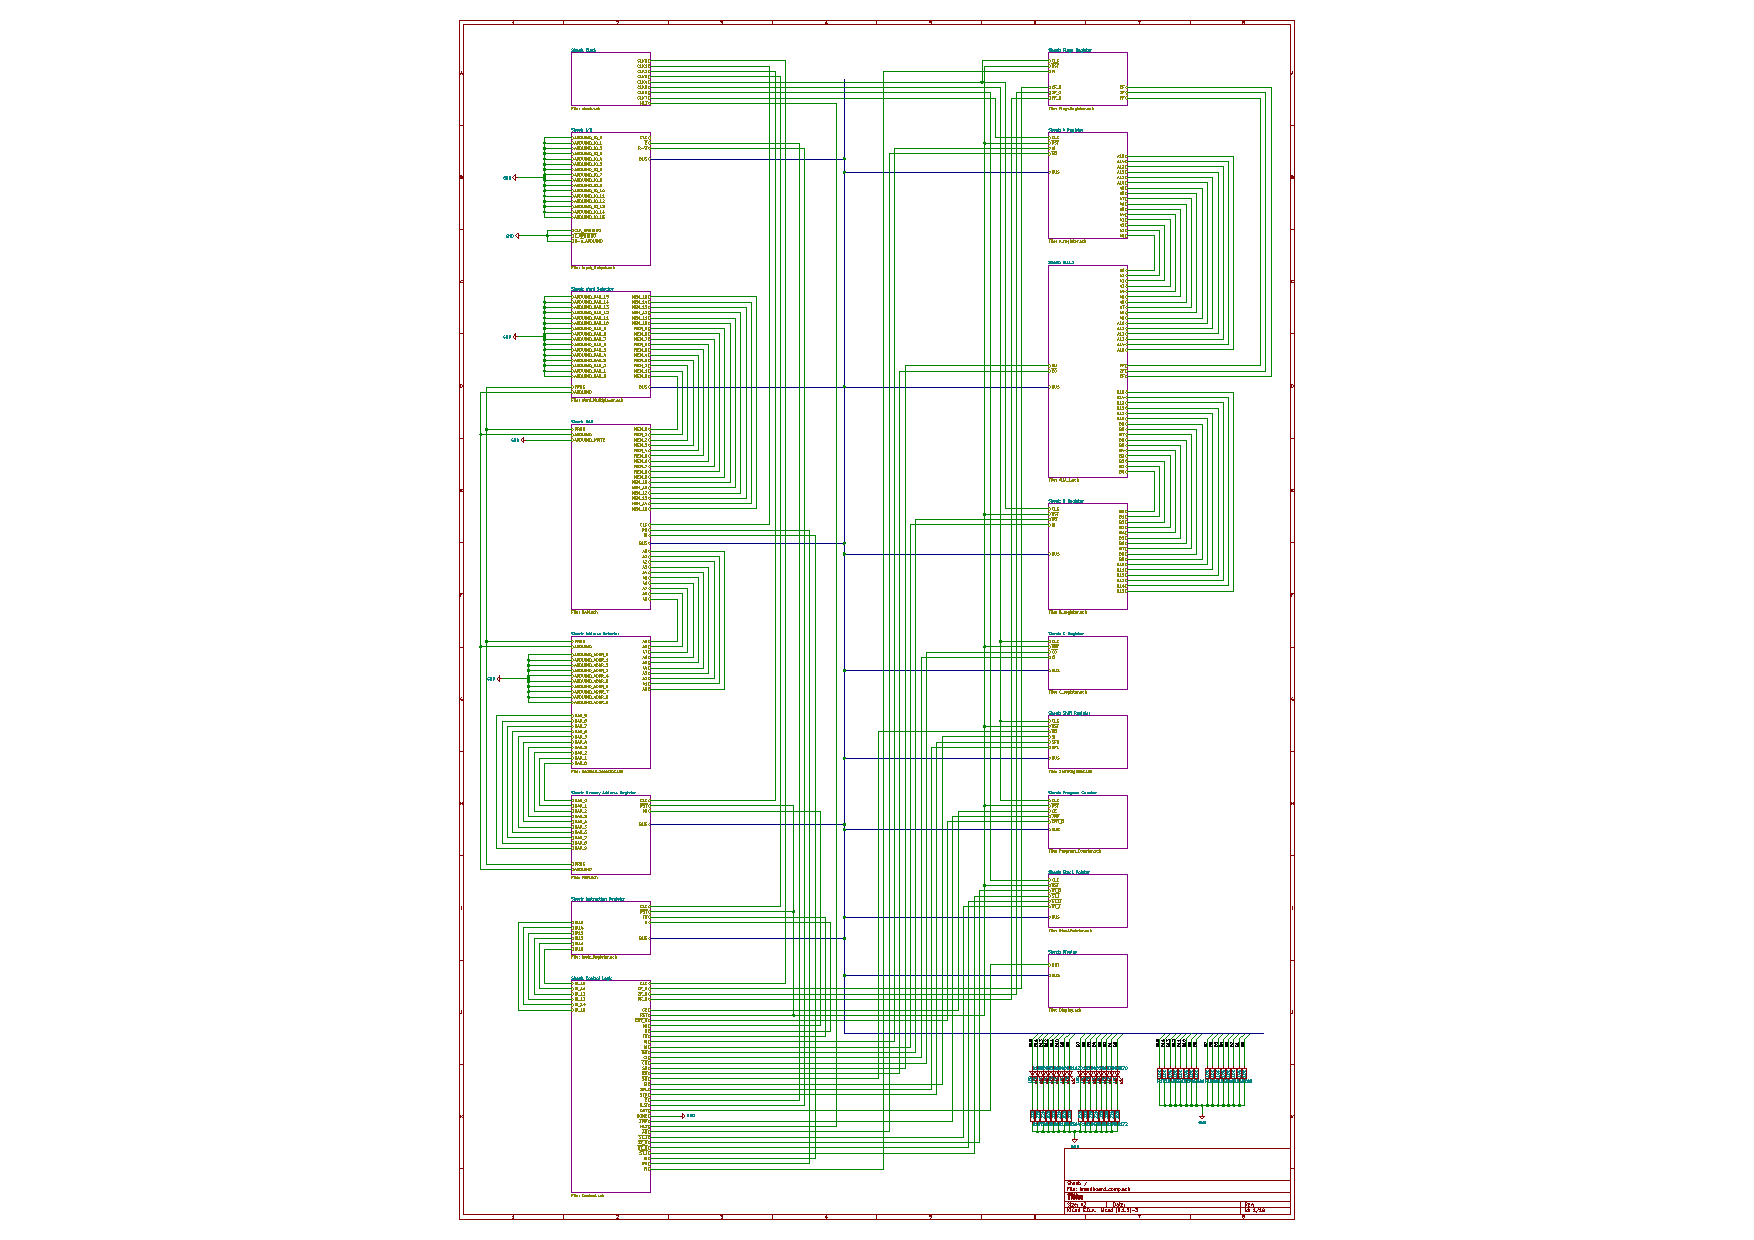
\includepdf[page={1}]{./pdf/kicad}
\clearpage

\paragraph{Clock} \ref{clock}
The clock module is very similar to the clock designed and built by Ben Eater \cite{eater2020clock}. It uses \emph{555 timers}
\cite{555} to generate a square wave which acts as the clock for the system. The \emph{555} is presented in all three most commonly
used configurations:
\begin{itemize}
  \item \emph{Astable: } it oscillates between to states (This 555 generates the main clock)
  \item \emph{Monostable: } it always ~~settles down`` to one state after a short period of time (used for the manual push-button
  clock mode)
  \item \emph{Bistable: } it has two states between which it can toggle (used for the toggle switch which goes from automatic to
  manual mode)
\end{itemize}
The clock-pulse generating \emph{555} is connected to a variable resistor which can be adjusted to increase or decrease the
frequency accordingly. A simple combinatorial circuit is used to select the appropiate clock signal and inhibit it if the \emph{HLT}
 (Halt) signal is active. The main addition to the Eater design is a \emph{74ls245 buffer} \cite{74ls245} used to amplify and
 isolate clock signals going to each module.

 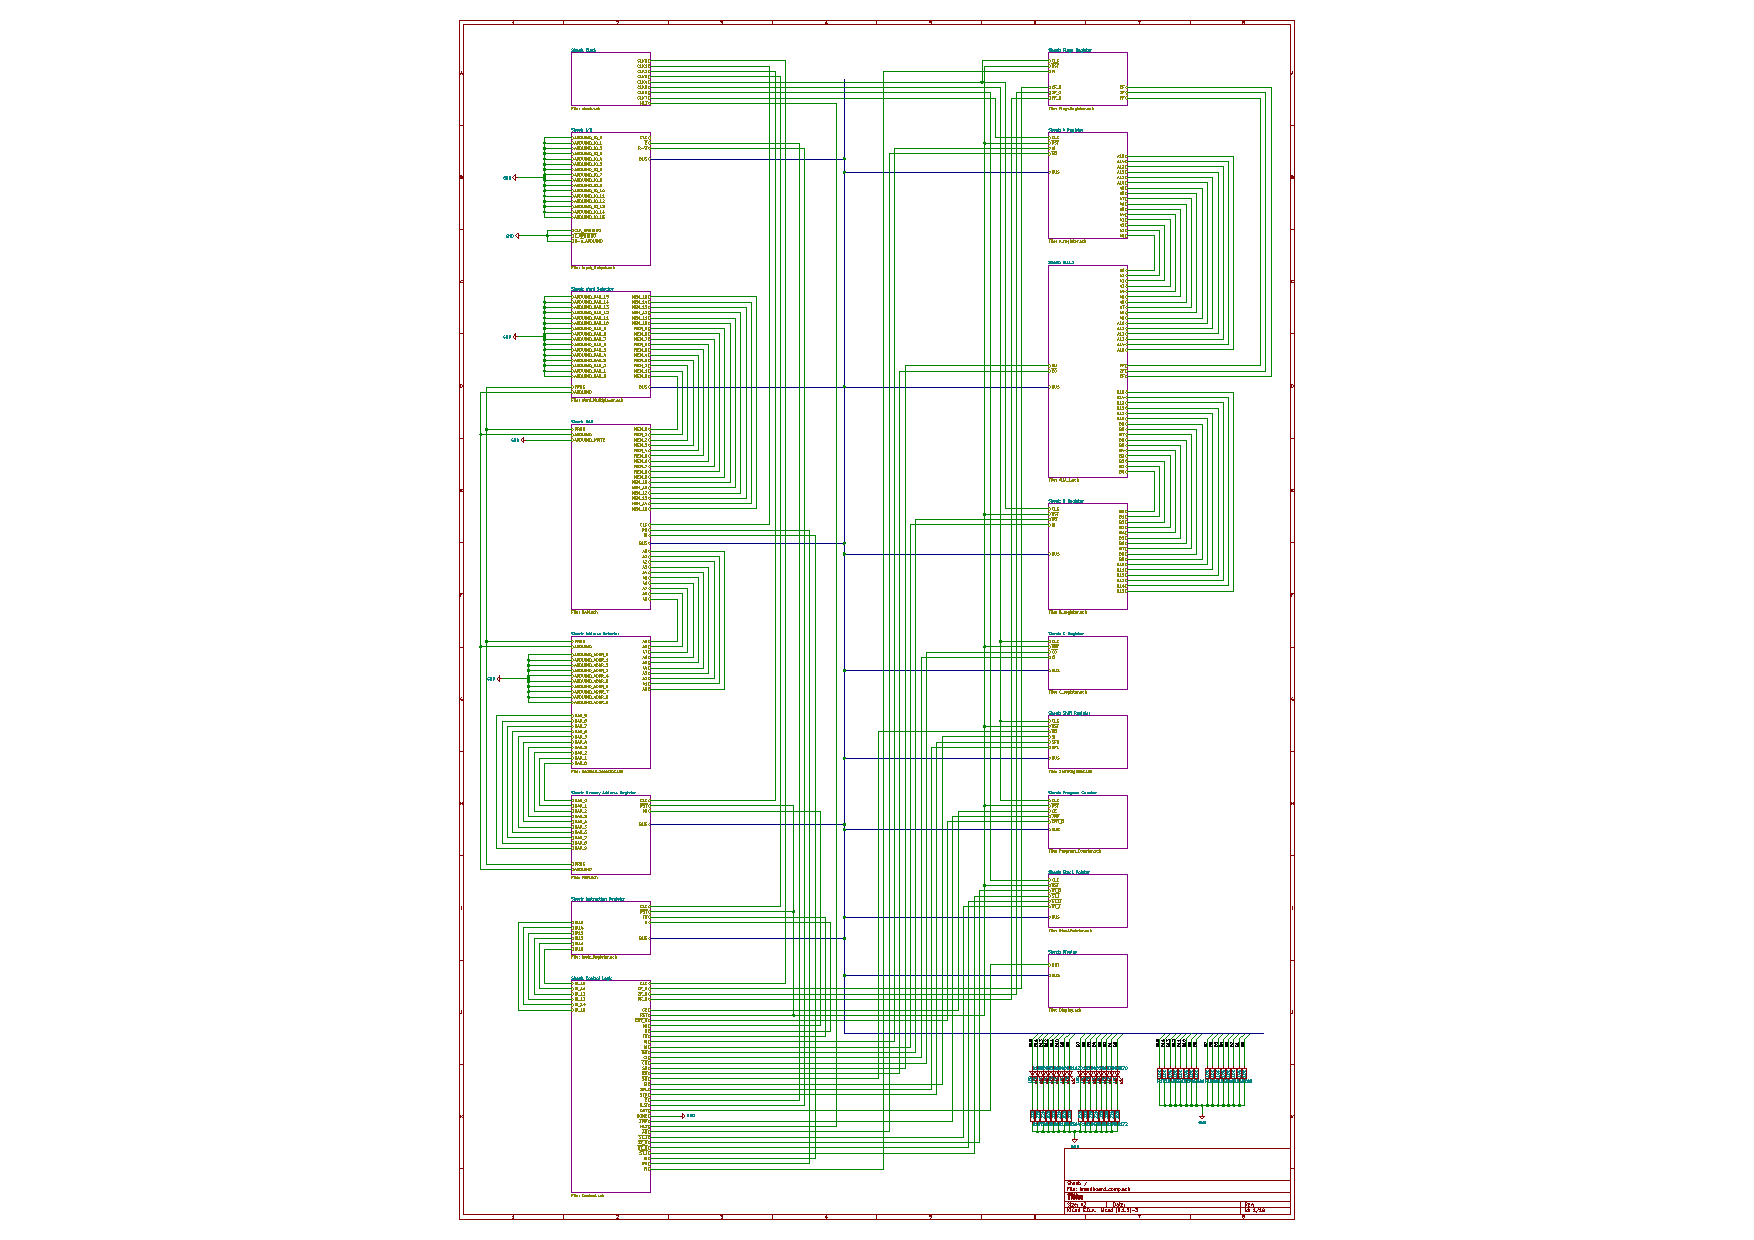
\includepdf[page={2}]{./pdf/kicad}

\paragraph{A Register} \ref{a-reg}
The A register consists of two \emph{74ls273} \cite{74ls273} 8-bit flip-flop chips and two \emph{74ls245} \cite{74ls245} buffer
interfaces to the bus. The buffers are \emph{tri-state} buffers, which means that they can pass through their input, either high or
low, or they can  disconnect their input from their output by putting themselves in a high-impedence state. This functionaility,
used across most modules which interface with the bus, is used to allow the register to assert its contents onto the bus when
reading from it (this happens when the \emph{$\overline{AO}$} signal is taken low). Writing to the register is handled by
ANDing together the \emph{AI} signal with the clock pulse. The contents of the A, which can be foud on the \emph{Q} pins, are
connected directly to the \emph{ALU} \ref{alu}.

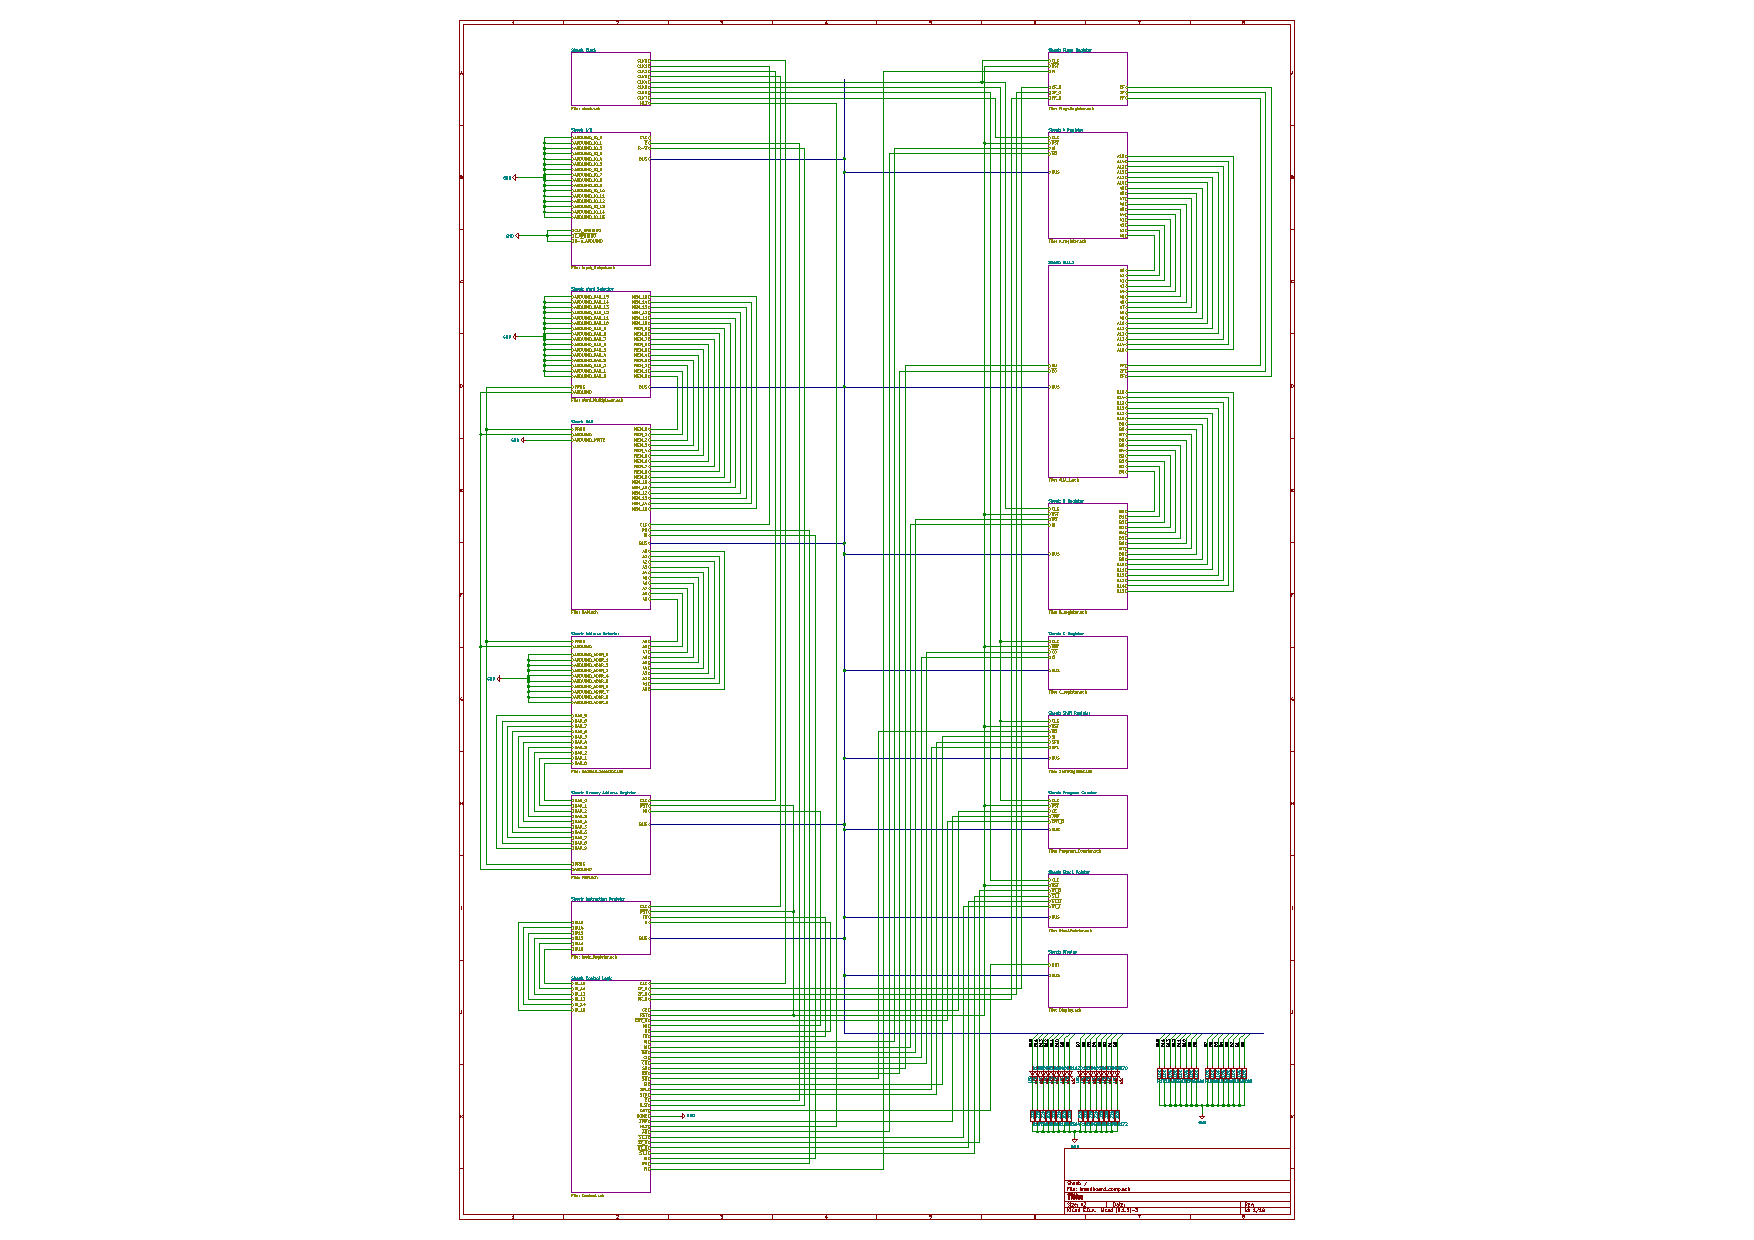
\includepdf[page={3}]{./pdf/kicad}

\paragraph{B Register} \ref{b-reg}
The B register is built essentially the same as the A register.

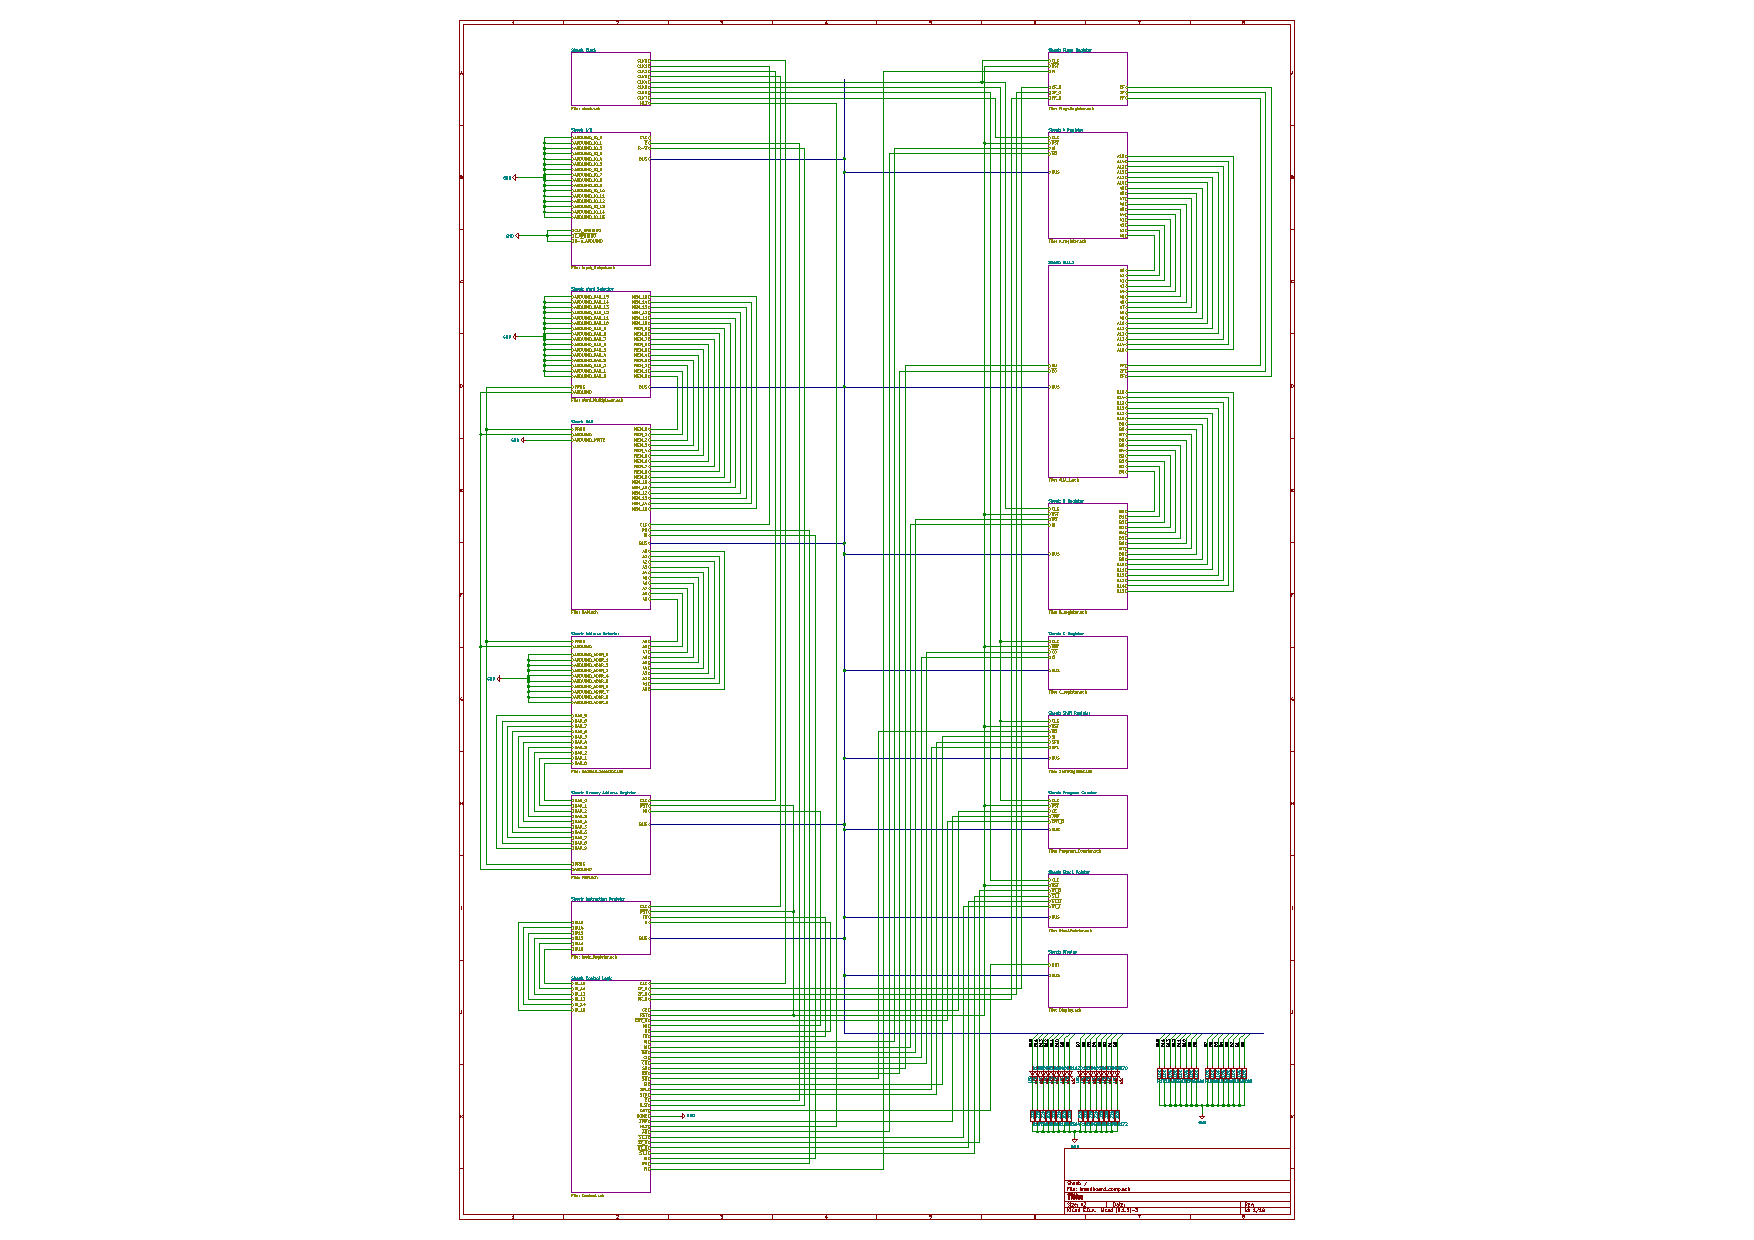
\includepdf[page={4}]{./pdf/kicad}

\paragraph{Arithmetic-Logic Unit} \ref{alu}
The \emph{ALU} has been designed around the \emph{74LS283} \cite{74ls283} chip. It contains a 4-bit binary full adder.
They can be chained together by connecting the Carry-Out of one chip to the Carry-In of the next chip. This way, by using 4
chips, a full 16-bit adder can be constructed. The A inputs are connected to the A register \ref{a-reg} and the B inputs
are conected to the B register \ref{b-reg}. The sum output is connect to two \emph{74LS245} \cite{74ls245} buffers which make the
connection to the data bus. To achieve subtraction functionality, the inputs from the B register are converted to two's complement
binary  notation, since subtracting a value equates to adding up the same negative value. To convert a positive binary value to a
two's complement negative value of the same magnitude, all 16 bits have to be flipped and then 1 has to be added to the number.
Flipping the bits is accomplished using the \emph{74LS86} \cite{74ls86} , which provides four independet XOR (exclusive or) gates.
By XORing each bit of the bit register with the value of the \emph{SU} control signal, each bit will just pass through the gate
if \emph{SU} is low and it will be flipped if \emph{SU} is high. Besides this, \emph{SU} is also connected directly to the Carry-
In Input of the first \emph{74LS283} full adder chip, to artificially add one to the final sum, representing the one which needs
to be added in for the two's complement form of the B register contents. \\
The \emph{ALU} also has three \emph{flag signals} which go out to the \emph{Flags Register} \ref{flags}. These are the \emph{Parity
Flag (PF)}, which represents the state of the lowest-significand bit of the sum, the \emph{Zero Flag (ZF)}, which is high if the
sum is 0 and low otherwise, and the \emph{Carry FLag (CF)}, which is set if the sum inside the \emph{ALU} cannot be expressed
within 16 bits. These flags can be used to make branching decisions based on the result of a calculation. The \emph{Carry Flag} and
\emph{Paritiy Flag} are straight-forward to obtain. The \emph{Carry Flag} is the Carry-Out pin of the most-significand adder
circuit. The \emph{Parity Flag} is the least significand sum pin of the least significand adder circuit. To calculate the
\emph{Zero Flag}, \emph{NOR} (inverted or) gates are employed on each pair of two sum bits. These gate can be found on the
\emph{74LS02} \cite{74ls02} chips. If any of the sum bits goes high, then the output of at least one \emph{NOR} gate will go low.
Subsequently, all \emph{NOR} outputs are ANDed together using successive \emph{AND} gates found on \emph{74LS08} \cite{74ls08}
chips. By using the and operator, if any one of the \emph{NOR} gates goes low, then the final output, which is the \emph{Zero Flag},
will go low. The only case where the \emph{Zero Flag} will go high is if all sum bits are 0.

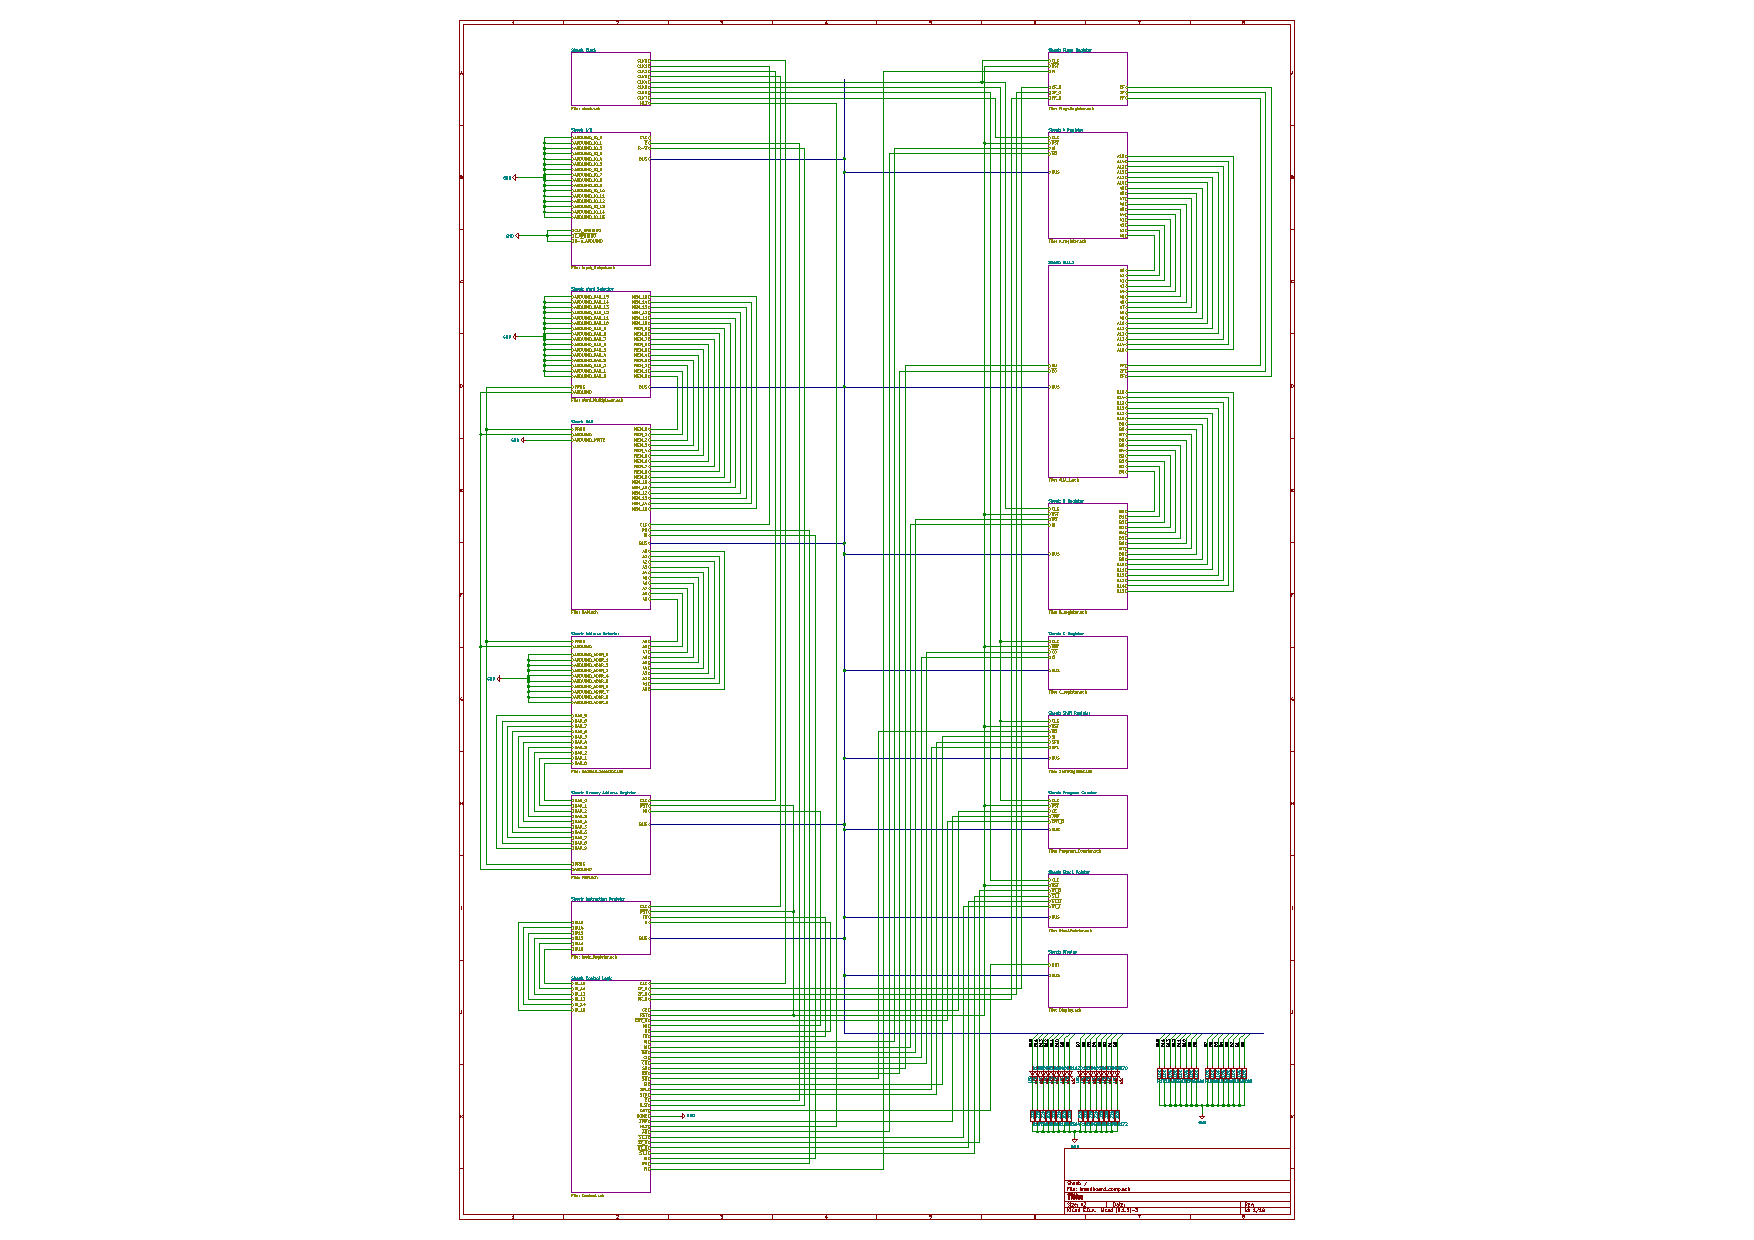
\includepdf[page={5}]{./pdf/kicad}

\paragraph{Flags Register} \ref{flags}
The Flags register consists of just one \emph{74LS273} \cite{74ls273} and some simple logic to handle the selective reads.
Allthough it is inneficient to use an 8-bit register to store only three bits, this design decision has been made because
the \emph{74ls273} is used in many other modeuls of the system and to avoid having to understand how another chip works and how
to use it.

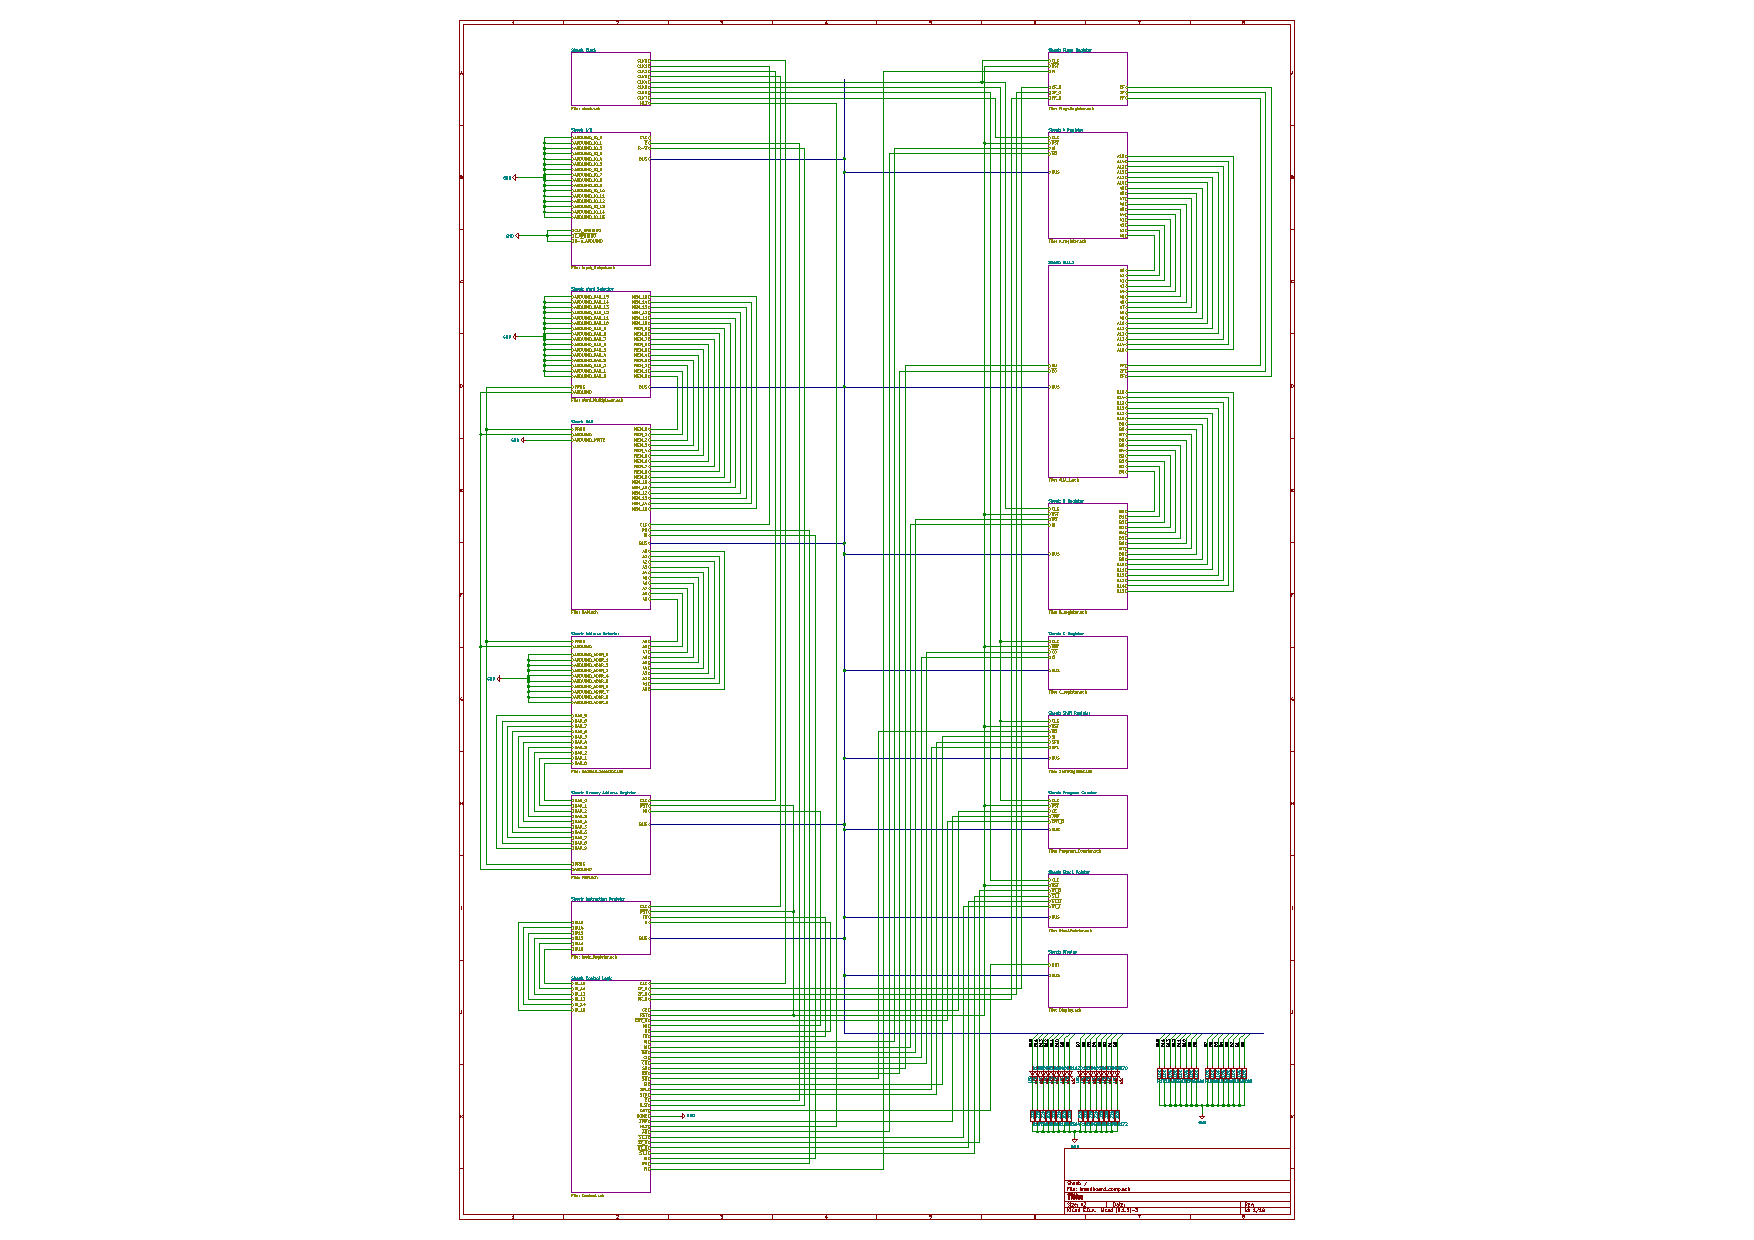
\includepdf[page={11}]{./pdf/kicad}

\paragraph{C Register} \ref{c-reg}
The C register is a general purpose 16-bit register built just like the A register \ref{a-reg} or the B register \ref{b-reg}.

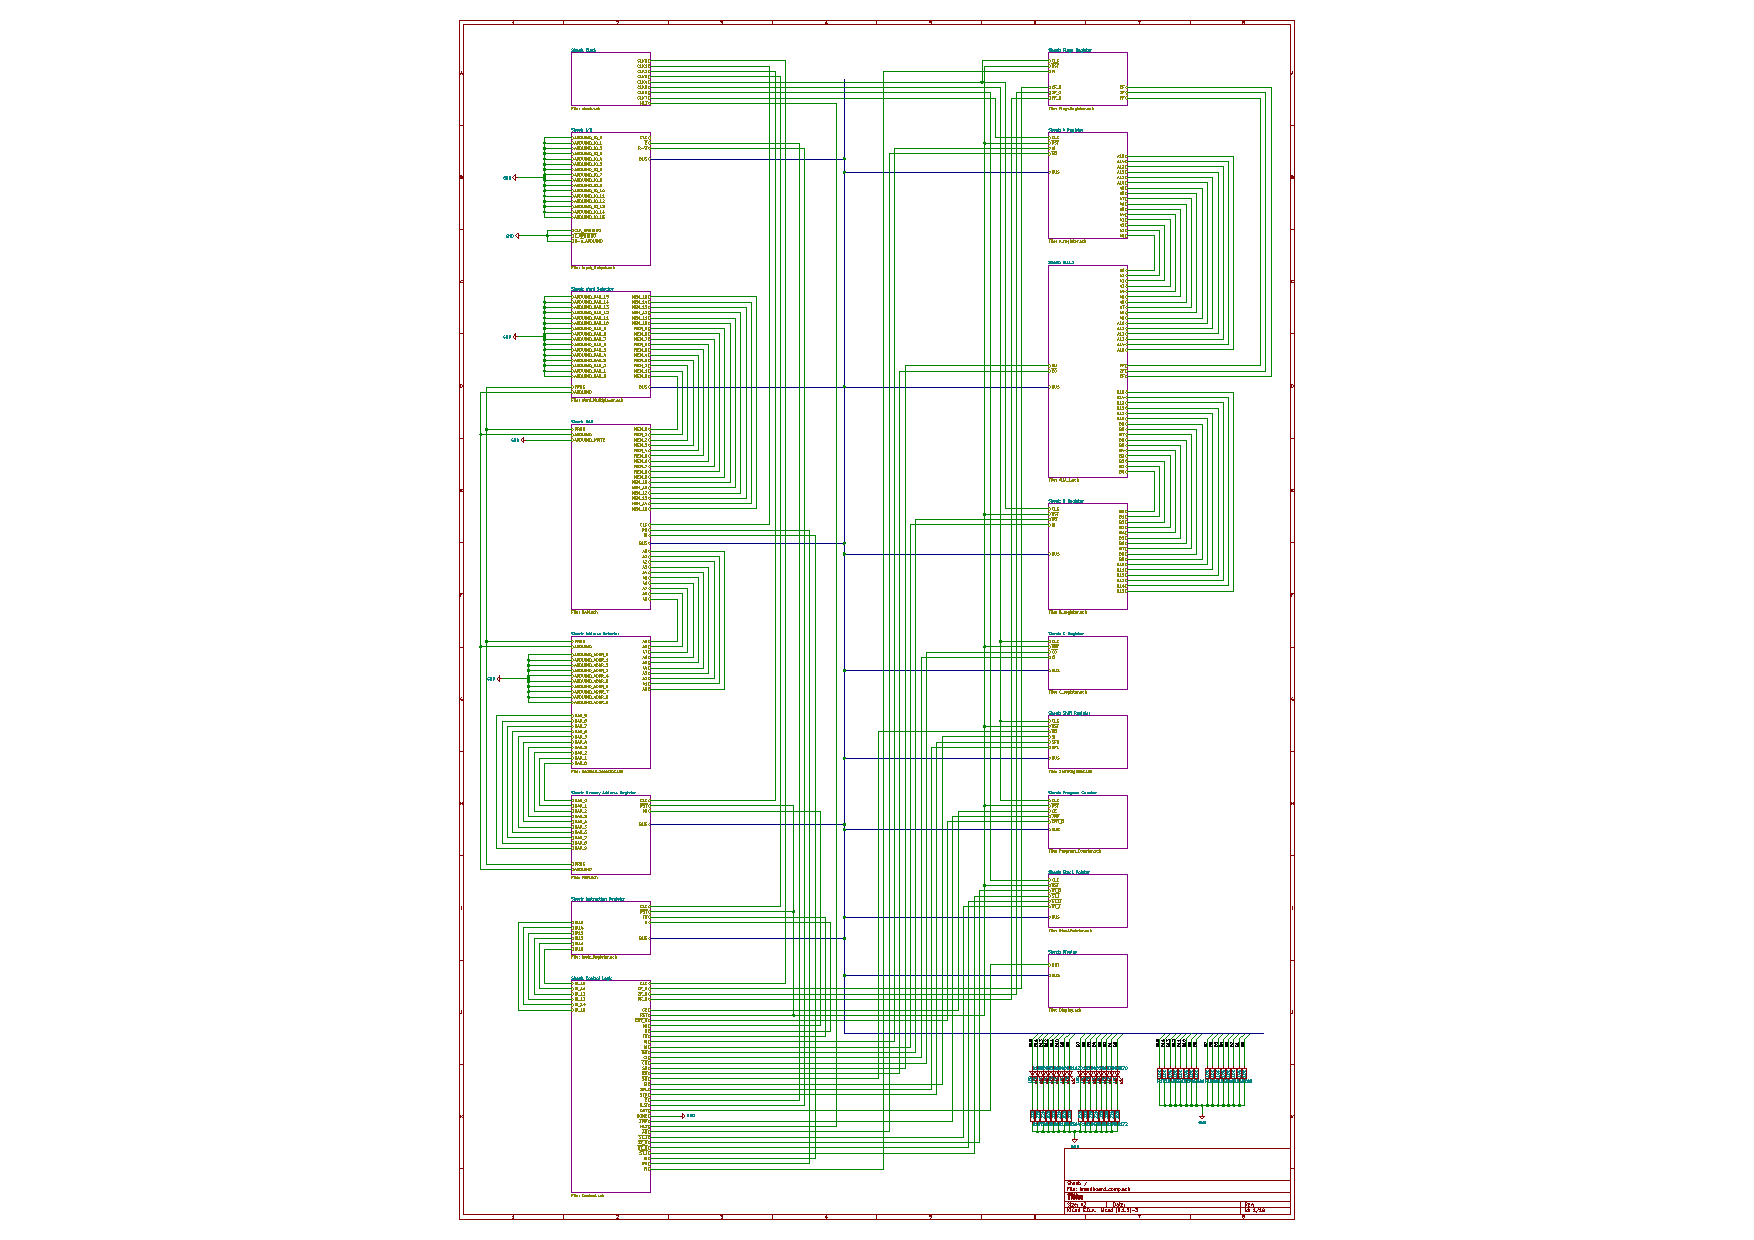
\includepdf[page={7}]{./pdf/kicad}

\paragraph{Shift Register} \ref{shift-reg}
For the design of the shift register, the \emph{74LS194} \cite{74ls194} was chosen. It is a 4-bit register which implements
bit shifting in both directions. Multiple \emph{74LS194} chips can be chained together to create a larger shift register by
connecting the Serial-Left and Serial-Right inputs of one chip to the data outputs of the chips to its left and right.
The chips have two control inputs, \emph{S0} and \emph{S1}. If both inputs are low, the register will do nothing on the next clock
pulse. If S0 or S1 is high, but not both, then a shift-right or a shift-left will occur, depending on which input is high.
If both are high, then a parallel load will occur. The data outputs of each chips are connected two two \emph{74LS245}
\cite{74ls245} chips to provided the interface to the data bus. The two control inputs are fed in from a simple combinatorial
circuit which converts the three control signals, \emph{SI}, or shift register in, \emph{SFL}, or shift left and \emph{SFR}, or
shift right, into the two lines which connect directly to the register chips.

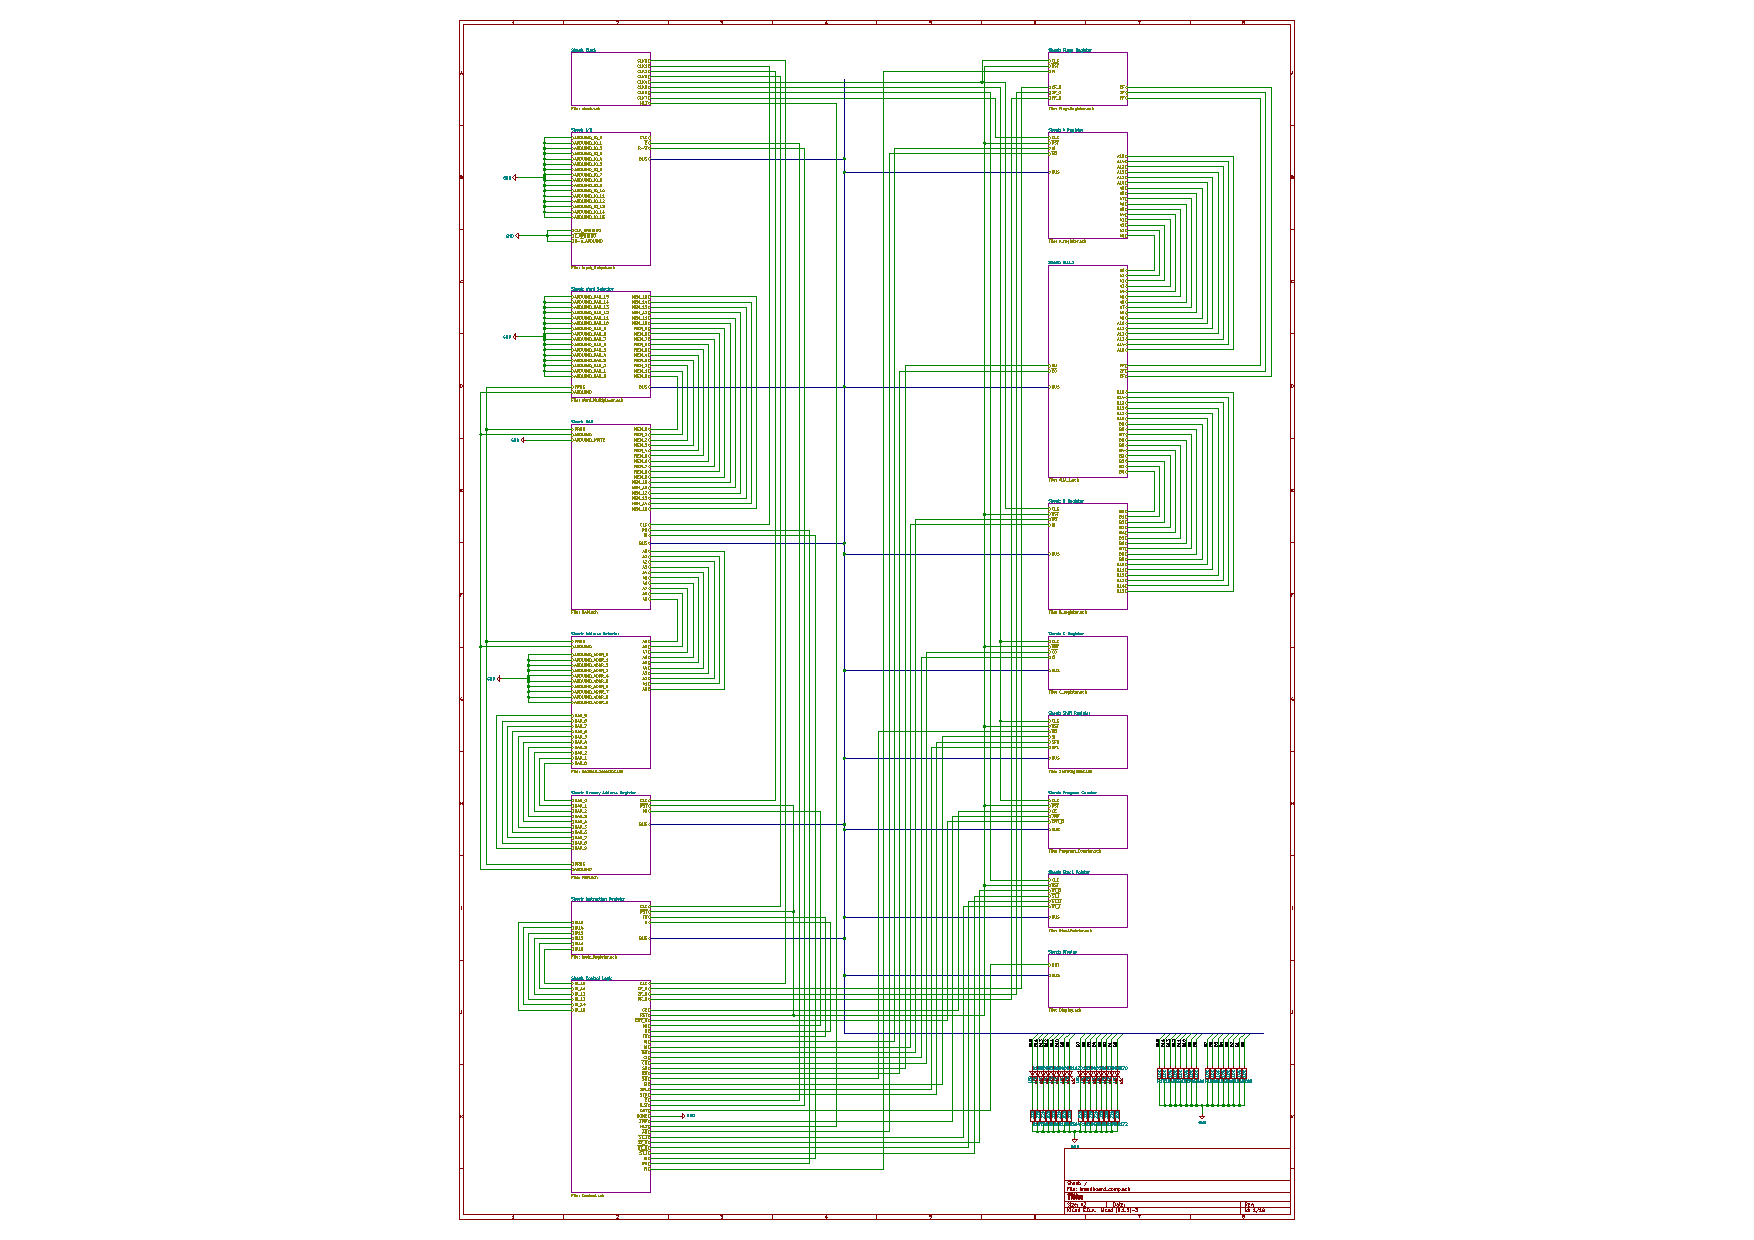
\includepdf[page={6}]{./pdf/kicad}

\paragraph{Random Access Memory (RAM)} \ref{ram}

% \chapter{Implementation}

\section{Section Heading}

% \chapter{Legal, Social, Ethical and Professional Issues and application of the BCS Code of Conduct}

\section{Legal, Social, Ethical and Professional Issues}

Taken into account the nature of this project and the way it has been conducted,
Legal, Social, Ethical and Professional Issues were unlikley to arrise. That being
said, it is important to go over each field separatley and show that no issues pertaining
to that field have appeard.

\begin{itemize}
  \item \emph{Legal issues: } The project did not pose any legal issues. There was no need
  to contact third parties, gain access to sensitive or classified information or any other
  activity which chould have created legal issues.
  \item \emph{Social or Ethical issues: } The project did not pose any social or ethical issues.
  There was no need to gather personal data, conduct surveys, create control groups or anything
  similar which could have affected the project and create social or ethical issues.
  \item \emph{Professional issues: } one professional issue presented itself early on in the
  project. As the project had a significant hardware component, the need to purchase the hardware
  became aparrent. The issue at hand was to determine who would fund the hardware needed for the
  project. After careful consideration, the decision was made to fund the project using personal funds
  so as to not have to be dependant on any other body or entity.
\end{itemize}


\section{Application of the BCS Code of Conduct}
The British Computer Society Code of Conduct \cite{bcs} applies to the project and, as such, the
project abides by this code of conduct. The main section where it is visible that this report aims to
abide by the BCS Code of Conduct is the ``Duty to the Profession'' section, point ``f'', as  well as
the ``Duty to the Profession'' interpretation. They state that a fellow abiding by the BCS Code
of Conduct shall ``encourage and support fellow members in their professional development'' and ``share
knowledge and understanding of IT and support inclusion of every sector of society.''. One of the main
goals of the project is to make computer architecture and design easier to approach from any
potential background and learn more about how computers work at a very low level. This is a reflection
of the directives cited above.

% \chapter{Results/Evaluation}

\section{Software Testing}

\section{Section Heading}

% \chapter{Conclusion and Future Work}

The project's conclusions should list the key things that have been learnt as a consequence of engaging in your project work. For example, ``The use of overloading in C++ provides a very elegant mechanism for transparent parallelisation of sequential programs'', or ``The overheads of linear-time n-body algorithms makes them computationally less efficient than $O(n \log n)$ algorithms for systems with less than 100000 particles''. Avoid tedious personal reflections like ``I learned a lot about C++ programming...'', or ``Simulating colliding galaxies can be real fun...''. It is common to finish the report by listing ways in which the project can be taken further. This might, for example, be a plan for turning a piece of software or hardware into a marketable product, or a set of ideas for possibly turning your project into an MPhil or PhD.

%%%%%%%%%%%%%%%%%%%%%%%%%%%%%%%%%
% References
%%%%%%%%%%%%%%%%%%%%%%%%%%%%%%%%%
\bibliographystyle{plain}
\bibliography{mybib}
\addcontentsline{toc}{section}{Bibliography}

%%%%%%%%%%%%%%%%%%%%%%%%%%%%%%%%%
% Appendices
%%%%%%%%%%%%%%%%%%%%%%%%%%%%%%%%%
% \appendix
% \include{Appendices/appendix}
% \chapter{User Guide}
\section{Instructions}
You must provide an adequate user guide for your software. The guide should provide easily understood instructions on how to use your software. A particularly useful approach is to treat the user guide as a walk-through of a typical session, or set of sessions, which collectively display all of the features of your package. Technical details of how the package works are rarely required. Keep the guide concise and simple. The extensive use of diagrams, illustrating the package in action, can often be particularly helpful. The user guide is sometimes included as a chapter in the main body of the report, but is often better included in an appendix to the main report.

% \chapter{Source Code}
\section{Instructions}
Complete source code listings must be submitted as an appendix to the report. The project source codes are usually spread out over several files/units. You should try to help the reader to navigate through your source code by providing a ``table of contents'' (titles of these files/units and one line descriptions). The first page of the program listings folder must contain the following statement certifying the work as your own: ``I verify that I am the sole author of the programs contained in this folder, except where explicitly stated to the contrary''. Your (typed) signature and the date should follow this statement.

All work on programs must stop once the code is submitted to KEATS. You are required to keep safely several copies of this version of the program and you must use one of these copies in the project examination. Your examiners may ask to see the last-modified dates of your program files, and may ask you to demonstrate that the program files you use in the project examination are identical to the program files you have uploaded to KEATS. Any attempt to demonstrate code that is not included in your submitted source listings is an attempt to cheat; any such attempt will be reported to the KCL Misconduct Committee.

\textbf{You may find it easier to firstly generate a PDF of your source code using a text editor and then merge it to the end of your report. There are many free tools available that allow you to merge PDF files.}


\end{document}
